%-----------------------------------------------------------------------
% Latex Thesis/Dissertation Template for Wright State University
%
% Written by Sean A. Mortara
% 28 June 2001
% Modified by Josh Mark
% 15 Dec 2011
% Later edits by Joseph C. Slater
%-----------------------------------------------------------------------
\documentclass[12pt]{report}

\usepackage{xcolor}
\usepackage{booktabs} % used for tables
\usepackage{multirow} % used for tables to merge multiple rows
\usepackage{bigdelim} % used for tables to set spacing
\usepackage{bigstrut} % used for tables to set spacing
\usepackage{graphicx} % used for includegraphics
%\usepackage{subfigure} % allows the use of subfigures
\usepackage{subcaption} % also allows the use of subfigures but not deprecated
%\usepackage[framed,numbered,autolinebreaks,useliterate]{mcode} % used to insert code
\usepackage{listings}
\usepackage{pgfgantt}
\usepackage{lscape}
\usepackage{listings}


%
%
%



%-----------------------------------------------------------------------
%  Modified fields
%-----------------------------------------------------------------------
\newcommand{\authorfirst}{Bradley}
\newcommand{\authorMI}{A.~}
\newcommand{\authorlast}{Schneider}
\newcommand{\degreefull}{Doc\-tor of Phil\-os\-o\-phy}  % force hyphenation at syllables if line breaks are required
\newcommand{\degreeshort}{Ph.D.}
\newcommand{\thesisordissertationlc}{Dissertation} % Make this uppercase
\newcommand{\dept}{Department of Computer Science and Engineering}
\newcommand{\institution}{Wright State University} % Doubting you will
                                % change this.
\newcommand{\thesistitle}{Bridging the Gap between Atomic and Complex
Activities in First Person Video using Fuzzy Inference} % Needes a line break
\newcommand{\bachdegreeshort}{B.S.} % Bachelor degree short
\newcommand{\bachinstitution}{Morehead State University} % Bachelor degree institution
\newcommand{\bachyear}{2012}% Bachelor degree year
\newcommand{\masterdegreeshort}{M.S.} % Bachelor degree short
\newcommand{\masterinstitution}{Wright State University} % Bachelor degree institution
\newcommand{\masteryear}{2017}% Bachelor degree year
%No spaces should be before or after this title.
\newcommand{\pdfsubject}{a short paraphrase of your title or focus of your thesis}
\newcommand{\pdfkeywords}{keyword 1, keyword 2, keyword 3, keyword 4}
\newcommand{\yearcomplete}{2020}
% set pdf file info
\usepackage{hyperxmp} % used to set pdf property info with \hypersetup command

%-----------------------------------------------------------------------
%  Thesis Advisor, Department Chair, Dean of Graduate Studies
%  I don't know why titles as separated... except in the one case at
%  the end.
%-----------------------------------------------------------------------
\newcommand{\thesisdirector}{Tanvi Banerjee}
\newcommand{\thesisdirectortitle}{Ph.D.}
\newcommand{\phdProgrameOrDeptChair}{Yong Pei} % CHANGE TO: Faculty M. Name FOR MASTER THESIS
\newcommand{\phdProgrameOrDeptChairEducation}{Ph.D.} % CHANGE TO: Ph.D., P.E. ETC
\newcommand{\phdProgrameOrDeptChairTitle}{Director, Computer Science and Engineering Ph.D. Program} % CHANGE TO: Chair, Department of Mechanical and \\ Materials Engineering FOR MASTER THESIS in MME


% COMMENT THE FOLLOWING 3 LINES FOR MASTER THESIS. PLEASE NOTE THAT FOR MASTER THESIS YOU SHOULD USE "\masterSignaturePage" AND FOR PHD DISSERATION "\phdSignaturePage" IN THE "approval sheet" SECTION.
\newcommand{\graduateSchoolDean}{Barry Milligan}
\newcommand{\graduateSchoolDeanEducation}{Ph.D.}
\newcommand{\graduateSchoolDeanTitle}{Interim Dean of the Graduate School}

%-----------------------------------------------------------------------
%  Final Examination Committee: Comment out the ones you don't need.
%-----------------------------------------------------------------------
\newcommand{\fecone}{Tanvi Banerjee, Ph.D.}

\newcommand{\fectwo}{Yong Pei, Ph.D.}

\newcommand{\fecthree}{Michael Riley, Ph.D.}

\newcommand{\fecfour}{Mateen Rizki, Ph.D.}

\newcommand{\fecfive}{Thomas Wischgoll, Ph.D.}

% If you have more committee members... good luck

% Modify this if needed for getting citations to "look right" according to your field. Read the natbib documentation on how to use this.
%\usepackage[round]{natbib}
%\usepackage{doublespace}

%=============================
%  Begin document!
%=============================
%
% Don't touch

% still don't touch.

% title sheet
\usepackage{WSUThesisTemplate/WSU}
\hypersetup{
                     pdfauthor={\authorfull},
                     pdftitle={\thesistitle},
                     pdfsubject={\pdfsubject},
                     pdfkeywords={\pdfkeywords},
                     }
% \normalem
\pagenumbering{roman}
\pagestyle{plain}
\rhead{\today}
\begin{document}
\maketitle
\doublespace\

% Still don't touch!!

%=============================
%  approval sheet
%=============================

\thispagestyle{empty}
\renewcommand\baselinestretch{2}
\begin{singlespace}
%\masterSignaturePage\newpage     % USE FOR MASTER THESIS
% You don't need both signature pages. Please comment out unnecessary lines in the .tex file. \newpage
\phdSignaturePage\newpage        % USE FOR PHD DISSERTATION
\end{singlespace}
%
%=============================
%  Abstract
%=============================
\newpage
\setcounter{page}{3}
\vspace{2in}
%
\begin{singlespace}
\begin{center}
  ABSTRACT
\end{center}
%
\noindent{\small{\authorlast, \authorfirst}.
		 {\degreeshort, \dept, \institution},
		 {\yearcomplete}.
		 {\sl \thesistitle}.}
\end{singlespace}
\vspace*{.5in}

\pdfbookmark[0]{Abstract}{Abstract}
%\phantomsection
%
%========================
% Start editing below.
%========================
Activities of Daily Living (ADL's) are the activities that people perform every day in their home as part of their typical routine. The in-home, automated monitoring of ADL's has broad utility for intelligent systems that enable independent living for the elderly and mentally or physically disabled individuals. With rising interest in electronic health (e-Health) and mobile health (m-Health) technology, opportunities abound for the integration of activity monitoring systems into these newer forms of healthcare.

In this dissertation we propose a novel system for describing ADL's based on video collected from a wearable camera. Most in-home activities are naturally defined by interaction with objects. We leverage these object-centric activity definitions to develop a set of rules for a Fuzzy Inference System (FIS) that uses video features and the identification of objects to identify and classify activities. Further, we demonstrate that the use of FIS enhances the reliability of the system and provides enhanced explainability and interpretability of results over popular machine-learning classifiers due to the linguistic nature of fuzzy systems.



%%%%%%%%%%%%%%%%%%
%-----------------------------------------------------------------------
%
%=============================
%  Table of contents, etc.
%=============================
%\renewcommand\baselinestretch{1.5}
\begin{singlespace}
\tableofcontents
\listoffigures
\listoftables
\end{singlespace}
%
%=============================
%  Acknowledgments
%=============================
% \newpage
% \thispagestyle{plain}
% \setlength{\parindent}{0em}
% \begin{center}
% {\huge Acknowledgment}
% \end{center}

% I would like to take this opportunity to extend my thanks to\ldots\  If you have multiple paragraphs, the first should not be indented to match the style of the rest of the thesis.

% \setlength{\parindent}{2em}
% Any additional paragraphs should be indented as such.  That ugly command before this, you don't need to keep doing that. Remember to thank your advisor and committee members. Probably your Mom, others as you wish. 
%
%=============================
%  Dedication
%=============================
% \newpage
% \thispagestyle{plain}
% \vspace*{3in}
% \begin{center}
% Dedicated to\\
% Somebody special (Wife, husband, girlfriend or boyfriend works well
% here.)
% \end{center}
%
%
%
%=============================
%  Begin Chapters
%=============================
\newpage
\setcounter{page}{1}
\pagenumbering{arabic}
\setlength{\parindent}{2em}

%================================================
\chapter{Introduction}
%================================================

%-------------------------
\section{Need for In-Home Monitoring}
%-------------------------
The number of people aged 65 and older in the United States is expected to reach 89 million by 2050, double the number of United States citizens in the same age group in 2011 \cite{Jacobsen2011AmericasPopulation}. As the elderly population continues to grow, so will the need to provide in-home care for the elderly. Elder care has traditionally been lacking qualified, certified practitioners and clinicians, and the demand for in-home health aides is very likely to exceed recruitment rates over this period of growth \cite{Rowe2016PreparingPopulation}. This will result in a growing deficit of qualified healthcare workers for in-home care, which will require the development of new models of healthcare delivery.

One response to this deficit of personnel is to leverage e-Health technology to provide in-home healthcare. In a 2005 report, the World Health Organization (WHO) defined e-Health as the “cost-effective and secure use of information and communications technologies in support of health and health-related fields, including health-care services, health surveillance, health literature, and health education, knowledge and research” and resolved to encourage long-term strategic plans to develop e-Health resources, noting that advances in technology have raised expectations for healthcare \cite{58thWorldHealthAssembly2005WHA58.28EHealth}. Since then, WHO has also formalized the idea of mobile-health, or m-Health, which is similar to e-Health but uses mobile technology. This includes in-home installation of sensors or imaging devices used to monitor patients with chronic illnesses \cite{WorldHealthOrganization2011MHealth:EHealth}. A recent survey of m-Health technology found that m-Health has been found as an effective way to monitor elderly patients suffering from dementia and cognitive disorders including screening for cognitive decline and promoting healthy habits in terms of physical activity \cite{Vazquez2018E-HealthReview}.

The need for in-home monitoring extends beyond caring for the elderly to monitoring individuals of any age who require assistance living independently due to a mental or physical disability or injury. In addition to the use of in-home monitoring for clinical purposes, it may be an important aspect of ubiquitous smart home systems. As more and more electronic devices are becoming internet-of-things (IoT)-enabled, including televisions, kitchen appliances, and security systems, the demand is growing for systems that automatically understand and react to users and their actions.


%-------------------------
\section{Activities of Daily Living}
%-------------------------
Activities of Daily Living (ADL’s) are defined as activities routinely performed in daily life, often for basic hygiene and personal care as well as food preparation, housekeeping, and other aspects of independent living. These activities have been studied since at least the 1960s \cite{LawtonAssessmentLiving} as an assessment for the ability to perform physical self-maintenance, especially among the elderly. Several scales of assessment have been proposed, each with the common purpose of evaluating the cognitive and physical capabilities of the subject \cite{LawtonAssessmentLiving, Bucks1996AssessmentScale, Carswell1993ActivitiesDisease}. In the clinical setting, it has been shown that the ability to independently perform ADLs is an indicator of the onset and progression of conditions such as Dementia and Alzheimer's disease \cite{Desai2004ActivitiesTreatment}.

The manual assessment of human activities is dependent on the ability for the subject to be observed, necessitating the use of either in-home visits by a clinician or visits by the subject to clinical laboratories. This can be challenging when considering the expense of home visits and the limited ability of elderly to travel and coordinate appointments. The use of technology through eHealth and mHealth applications to monitor and observe ADLs in a home environment can greatly reduce the impact to both the subject and clinician by providing an unobtrusive, automated method of gathering activity data.

A challenge to implementing automated activity detection and recognition systems is the need for a formalized model defining each activity under observation. The ability to recognize activities as they occur comes very naturally for humans, but it is much more difficult to define for a machine. Human activities are defined in overlapping temporal and semantic spaces. That is, one higher-level activity may include the performance of several lower-level activities at the same time. Thus the definition of these activities may be subjective to the observer. 

For example, a subject may perform the high-level activity of preparing breakfast, which involves many actions and movements in a sequence over a significant period of time. Within the action of preparing breakfast, the subject may have accomplished the lower-level activity of making toast, and within that activity the subject may have accomplished the lower-level activity of inserting bread into the toaster. The chain of activities may continue decomposing all the way down to the activity of picking up a bag of bread. Figure \ref{fig:activity_scale} illustrates several possible activities involved with this scenario and places them on a scale of increasing complexity. Understanding the same or overlapping activities at all of these levels is crucial to a fully functioning activity monitoring system.

\begin{figure}
    \centering
    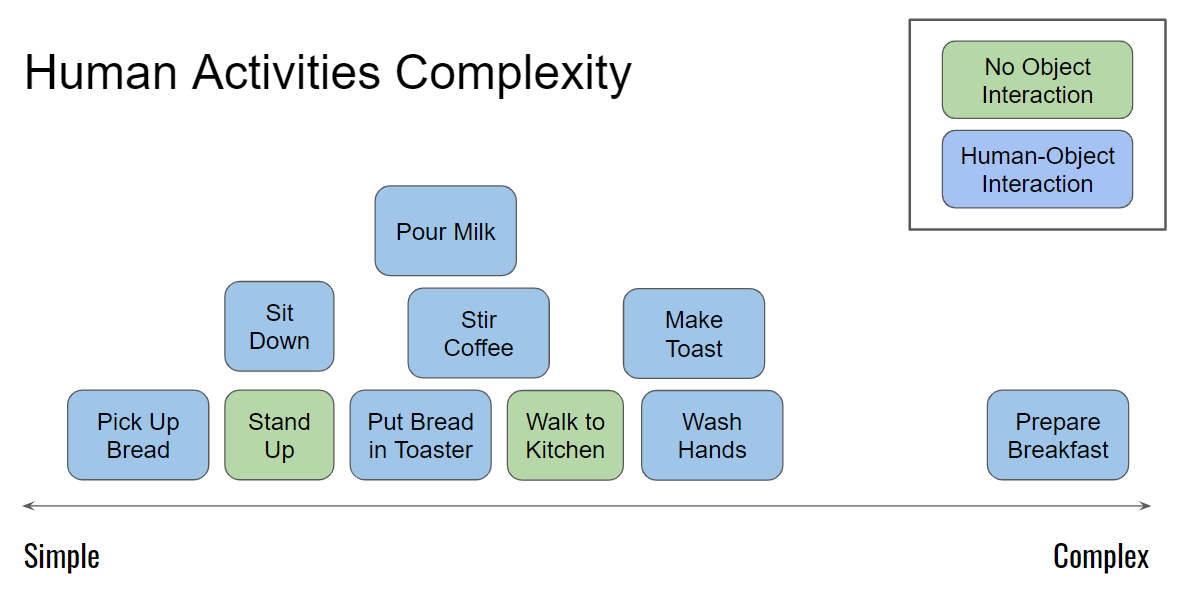
\includegraphics[width=\linewidth]{figure/activity_scale.png}
    \caption{Example of activities with varying spatio-temporal complexity which may occur during the larger activity of preparing breakfast.}
    \label{fig:activity_scale}
\end{figure}


%-------------------------
\section{Research Goals}
%-------------------------
\emph{Research Question 1: Can wearable sensors be used to unobtrusively monitor activities of subjects in a semi-structured environment?}
A desired outcome of this work is to provide evidence that a system based on wearable sensors may be used in the home (i.e. not in a clinical setting or laboratory) to provide continuous monitoring of activities of daily living. The outputs of the system provide data on activities and patterns of activities to inform clinicians on possible changes in the health and wellness of the user. Data collected at clinical laboratories is temporally sparse and involves scripted movements, bringing into question the validity of the data for assessing the subject’s ability to perform the actions in a natural environment; by contrast, the data collected by in-home monitoring will show a more complete look into the subjects’ abilities to perform activities on a day-to-day basis.
Early work was focused on detecting and measuring gait in controlled and semi-controlled environments \cite{Schneider2017PreliminaryProcessing, Schneider2019ComparisonEnvironments}. While results were achieved with uninterrupted gait sequences of several meters, it was clear that long uninterrupted gait sequences are uncommon in many daily activities, which include starts and stops and navigation around household objects. For this reason, the ultimate focus of this work is on object interactions rather than gait, as object interactions provide a much richer context for activities that are being performed.

\emph{Research Question 2: Can features extracted from first-person videos recorded in subjects’ homes be used to categorize different interactions with objects?}
The use of object interactions to determine activities has been popular in recent automated activity recognition and classification systems \cite{Pirsiavash2012, Sudhakaran2018, Nakatani2018PreliminaryKnowledge, Wang2018, Gokce2019HumanPairs}. Many in-home ADL’s are at least partially defined by interactions with certain objects. For example, knowing that a subject is interacting with a remote control should reveal that the subject is interacting with a television or other electronic device. The search space of candidate activities can be greatly culled by knowing which objects are involved. A desired outcome of this work is to exploit a combination of video and object features to characterize different interactions with objects.
Building on an initial set of features from previous work with gait, an initial baseline set of features was identified for categorizing object interactions. In addition to the location of objects, this set of features was heavily dependent on optical flow features to identify changes in object location and color features to identify changes in the appearance of objects. Additional experiments are needed to extend and refine this set of features and the resulting Fuzzy Inference System (FIS) that was developed, but the initial work proved the feasibility of using first-person video features to categorize object interactions.

\emph{Research Question 3: Can the activity identification system a) accurately describe activities and b) handle uncertainty in the results better than current state-of-the-art methods?}
While much recent work has been done on using deep learning and neural networks to identify human activities in video sequences (such as run, walk, sit down, throw, turn on faucet, open refrigerator, etc.) \cite{Abebe2016, Ozkan2017, Li2016}, there are two major drawbacks to the current deep learning trend:
\begin{enumerate}
    \item The networks must be trained to recognize a very specific set of actions. To date, most work involving neural networks has been against small sets of precisely defined and scripted activities, limiting practical applications.
    \item Since deep learning requires no features to be identified/extracted, the use of these technologies in isolation provides no ability to explain the outcome – only to identify it. That is, when the network fails to provide the correct answer, there is no explainability of the result or the misidentified activity.
\end{enumerate}

We propose the use of fuzzy logic to address these limitations. Many activities are very similar in their basic movements and absolute identification may become difficult as the set of activities grows. If an unknown activity occurs, fuzzy outputs may still provide some insight into the activity or similar activities. This is an advantage over machine learning approaches which will simply fail to identify the behavior. The simplicity of a fuzzy system can be seen in different lights; our goal is to show that the simpler fuzzy model is capable of providing a rich description of activities. In the course of attempting to identify an activity, the fuzzy system will produce interpretable fuzzy variables (as opposed to unexplainable deep learning features) which describe actions in the scene  - for example, a specific object in the scene is being interacted with and the subject is manipulating the shape of the object. While the overall activity might be unidentified, a good amount of information may still be taken away from the fuzzy system.


%-------------------------
\section{Thesis Statement}
%-------------------------
This dissertation proposes to bridge the gap between in-home activity monitoring leveraging an object recognition framework and using a fuzzy linguistic framework to handle uncertainty in complex movements between humans and objects in an in-home unstructured setting.


%================================================
\chapter{Related Work}
%================================================
This chapter contains a summary of the existing body of work related to the objective of describing activities occurring in first person video. The related work varies based on several factors - the types of activities detected, the sensors used to detect the activities, and the computational intelligence methods used to convert sensor data into activity information. The chapter is organized into sections based on these factors. Each section provides an overview of the variation seen within the related work with respect to the given factor.

\section{Activities Being Detected by Vision Sensors}

A number of activities have been found in related work on detecting and classifying activities using vision sensors. These related works were grouped into three categories, and discussion of the types of activities follows below:
\begin{enumerate}
\item Anomaly Detection, 
\item Full-body Activities, and
\item Partial-body Activities.
\end{enumerate}

\subsection{Anomaly Detection}

A subset of related work focuses on the detection of anomalous activities. Each of these systems used full-body views of subjects from third-person vision sensors combined with computational intelligence to observe an environment and determine when either an unexpected activity occurred, or when an activity occurred in an unexpected way. Systems detecting such anomalies focus on actions that do not fit expectations based on previous observations, but do not often focus on describing precisely what these anomalous actions are - just that they are unexpected.

In \cite{Beleznai2012}, a vision sensor monitored a pedestrian area and used motion history images to identify activities that were determined to be anomalies, such as vehicles entering the space, by means of clustering. This method approximated the spatio-temporal distribution of activities that occurred frequently and detected activities that did not fit that distribution. Another outdoor environment - a loading dock - was monitored for anomalous activities in \cite{Hamid2005}. Activities were represented as n-grams of events and a distance metric based on these n-grams determined the dissimilarity between activities. Anomalous activities that were discovered included a truck leaving the dock with its door open and an unusual number of people unloading a truck. 

Anomalous activity detection was also found in indoor environments. Fuzzy membership functions were used to captured several parameters of indoor human activities (location, time, perceived area of subject) from an omni-directional vision sensor and output a fuzzy determination of how "normal" each activity was \cite{Seki2009}. \cite{Yiping2006} presented a similar experimental setup with an indoor omni-directional vision sensor seeking to detect anomalous activities, but used Gaussian models of time and space to determine whether an activity was normal.

\subsection{Full-body Activities}

While detecting anomalies is useful for some applications, detecting the occurrence of a specific pre-defined activity is important for many applications. In the following reviewed studies, various vision sensors recorded subjects’ full bodies to detect specific activities using a variety of computational intelligence. These works have the goal of detecting a specific set of activities and differentiating the occurrence from other activities. These related works are able in the best case to exploit full third-person views of the subjects which provide a maximal amount of input information about both the subject and surrounding environment.

One such study described a system designed to detect a single activity (or a single \textit{type} of activity) - falls \cite{Banerjee2014}. This work focused on applications in elderly living facilities , where timely detection of falls is critical.  It compared the use of three different vision sensors in the same facility and was shown to be capable of detecting three fall-related activities - being upright, sitting, and being on the floor.

Another two related works were focused on using full body video sequences to detect activities in a medical setting. These environments, such as a trauma unit or patient room, may be very busy with doctors and nurses, and activities may be happening frequently or simultaneously. Because of this, both of the reviewed studies required systems capable of monitoring several subjects at the same time to identify activities \cite{Chakraborty2013, Bloisi2009}. The systems were focused on outputting activity information for a set of multiple actors in the scene, providing a summary or log of activities that may assist in the coordination of medical actions such as performing chest compressions, intubation, or checking pulse.

Many related studies which used full-body views from vision sensors were focused on detecting indoor activities of daily living. While the specific sets of activities varied somewhat from study to study, each of these were deployed in home-like environments and detected daily activities such as sitting on a sofa \cite{Figueroa-Angulo2013}, eating dinner \cite{Yao2016}, or reading a book \cite{ElHelw2009}. The sets of activities are pre-defined in each case (i.e. the system is trained to recognize a specific limited set of activities), and the works all make use of scripted training and test datasets. 

\subsection{Partial-body Activities}

A third class of related work focused on detecting activities using vision sensors with visibility of only part of the subjects’ bodies. These limited views often complicate activity detection since the entire posture of the subject is not able to be known by the system. However, the trade-off usually comes with improved usability, portability, or some other convenience to the user. For example, applications using wearable hardware are better able to integrate into all aspects of the user's daily routine.

A fall detection system based on a wearable camera was described in \cite{Mahabalagiri2013}. This work differed from \cite{Banerjee2014} in that it used only a partial view of the subject’s body, since the camera was worn on the torso. This system was capable of detecting a set of three activities similar to the full-body fall detection work, including sitting down, lying down, and falling.

Several studies applied partial-body views from a vision sensor to detect speaking activities. These studies were concerned with identifying speakers in multi-user or noisy environments, citing use-cases such as human-robot interaction \cite{Yoshida2010, Lim2009} and video calling \cite{Savran2018}. Though the recognition of the audio is important in each of these cases, the vision sensor provides valuable information for detecting the beginning and continuation of a speech activity, based on the movement of the subjects’ mouths. In these studies, the detection of activities would not necessarily benefit from knowing the full-body posture of subjects, and the closely focused view of the face was preferred for the enhanced details.

Similarly, studies were discovered which used partial-body views to detect activities while driving. These studies had a similar goal of detecting drivers’ actions while the car was in motion. These activities only require knowledge of the upper body posture. One study sought to build an understanding of actions that occur as the driver completes maneuvers such as turning or approaching an intersection \cite{Martin2017}. The other study was concerned with detecting both driving activities (steering, operating the shift level) and non-driving activities (eating, using cell phone) \cite{Zhao2012}.

As expected, many reviewed papers described systems which used partial-body views from a vision sensor to detect activities of daily living. In these cases, the vision sensor was attached to the subject, either a human or a robot, and computational intelligence was applied to make a determination of the current activity being performed \cite{Li2016, Wu2007}. Due to the positioning of the vision sensors, these studies have only a partial-body view of the subject. Unlike the studies detecting daily activities from full-body views, the partial-body view does not provide the visual information to determine the subject’s complete posture. These studies choose instead to exploit the information of specific objects \cite{Pirsiavash2012, Wu2007, McCandless2013, Nakatani2019} or other people within view \cite{Li2016} to detect the occurrence of an activity.

\subsection{Discussion}
Our results reveal a considerable degree of diversity in the types of activities to which activity detection via vision sensors and computational intelligence has been applied. Overall, the most common type of detected activities were indoor activities of daily living \cite{McIlwraith2009, Wu2007, Yao2016, McIlwraith2008, ElHelw2009, Rowe2007, Figueroa-Angulo2013, Mahabalagiri2013, Ong2013, Li2016, McCandless2013, Nakatani2019}. However, we also found results focused on detecting activities in medical settings \cite{Chakraborty2013, Bloisi2009}, in vehicles \cite{Zhao2012, Martin2017}, in the workplace \cite{Hamid2005}, and interactions with robots \cite{Yoshida2010}. A conclusion may be drawn that the vision and computational tools discussed have broad utility to intelligent systems which must understand the actions of users, regardless of the particular domain, setting, or application of that knowledge.

A drawback to the diversity of the activity domains in our results is that it remains difficult to draw direct comparisons between methods which have seen success. A vision-based system which performs well inside of a home may not perform well when deployed to detect activities in an outdoor work environment. Even within the same activity domain, we did not see a standard dataset emerging to provide a common baseline. In most of the studies, a new dataset was created, and little information was provided on how these datasets were captured. Further, datasets are typically gathered specifically for the evaluation of the system rather than from a truly operational deployment of the system.


%================================================
\section{Types of Vision Sensors}
%================================================
Our analysis revealed that several types of vision sensors have been used for activity detection. These sensors generally fell into the following four categories: 
\begin{enumerate}
    \item traditional fixed RGB vision sensors,
    \item fixed RGB-depth vision sensors,
    \item wearable RGB vision sensors, and
    \item wearable RGB-D vision sensors
\end{enumerate}
    
In some cases, several different devices were used either in concert or separately to provide the best results. The following subsections discuss the use of each of these types of hardware.

\subsection{Fixed RGB Vision Sensors}

Traditional RGB cameras come in a variety of styles, configurations, and sizes, and have been a frequent choice for vision-based activity recognition applications. The vast majority of related work incoporated one \cite{Yoshida2010, Savran2018, Beleznai2012, Wu2007, Seki2009, Yiping2006, McIlwraith2008, ElHelw2009, Rowe2007, Lim2009, Chakraborty2013, Zhao2012} or more \cite{McIlwraith2009, Bloisi2009, Martin2017, Hamid2005} fixed (i.e. non-mobile) RGB vision sensors. In each of these studies, the vision sensors were statically deployed in the environment within which the recognized activity is taking place, providing a third-person view of the subject(s). Within the category of stationary RGB cameras we see variation amongst the types and number of devices used, depending on the specific challenge being addressed.

One challenge that researchers face when using fixed (stationary) RGB vision sensors is a limited view of the environment, either due to a limited view angle or due to occlusion by objects. However, some researchers have been able to alleviate this issue. For example, some studies used multiple cameras simultaneously to provide a more complete view of the monitored environment. In \cite{McIlwraith2009}, a camera network was used to provide a comprehensive view of several seating stations within one room. The system mimics a home environment where activities such as dining, studying, and reading may be expected to occur in distinct locations. Individual camera nodes may provide sub-decisions, but communication between all nodes leads to a final result. Other studies that used multiple cameras examined differing use cases. For example, in \cite{Hamid2005} multiple cameras were deployed with partially overlapping viewpoints in order to provide complete coverage of activities that transpired in a loading dock. This allowed detection of multiple activities occurring in parallel at a given time.  Multiple cameras were also used in \cite{Martin2017} to provide detailed images of the face and hands of a subject driving a vehicle to analyze the coordination of the head and hands while maneuvering the vehicle. The cameras were positioned to optimally capture the relevant areas of the subject while excluding irrelevant details such as the dashboard or the passenger section of the car.

Our investigation also showed that researchers have found it possible to achieve an enhanced perspective without the use of multiple cameras. Two related studies incorporated omni-directional vision systems into the design of their activity recognition systems \cite{Seki2009, Yiping2006}. These cameras map a complete 360 degree view onto a typical two-dimensional intensity image, providing full monitoring of an area with a single hardware device, typically mounted overhead in the center of the space. Though this results in a distorted image due to the 360-degree perspective, the image may still be processed and human postures are still reliably discernable \cite{Seki2009}. A similar single-camera experimental setup is shown in \cite{Yiping2006} to effectively monitor an entire panoramic view of a room. The omni-directional vision device is capable of monitoring activities occurring in a seating area and four areas of entry or exit to other rooms.

A challenge in detecting activities with fixed RGB vision sensors is the lack of depth information from the scene. That is, only two dimensions of data are recorded, leaving out potentially valuable information about the movement and positioning of objects. However, traditional RGB cameras (which do not directly record depth information) can recover approximate depth information when used in pairs as a stereo camera. A depth dimension may be constructed by comparing the perspective of each camera given the predetermined distance between them. Two of the studies included in our review take this approach \cite{Lim2009, Bloisi2009}. In \cite{Bloisi2009}, depth information from a stereo camera is exploited to detect the background in each frame and subsequently remove it, leaving only foreground objects for consideration in activity recognition. Depth information from stereo cameras has also been used to determine distances between multiple subjects in the same area \cite{Lim2009}. The precision afforded by the depth information allows for improved facial tracking and differentiation between subjects in closer proximity to one another, improving the overall ability to differentiate the active speaker.

\subsection{Fixed RGB-Depth Vision Sensors}

As previously discussed, traditional RGB vision sensors record only a two-dimensional mapping of the three-dimensional environment. This is an important limitation because it is not possible to reconstruct the third dimension with high accuracy without the use of a standard vision system that integrates multiple vision sensors to provide different perspectives of the same area (i.e. a stereoscopic camera).

An alternative approach to providing depth information from a stereoscopic RGB vision sensor system is to use an RGB-Depth vision sensor. These sensors incorporate a traditional RGB camera, an infrared (IR) camera, and an IR projector. The IR projector projects a pattern of IR light onto the scene which is recorded by the IR camera to determine depth. The depth measures are combined as an extra channel of information with the image captured by the RGB camera. Several studies within our sample used RGB-D vision sensors \cite{Banerjee2014, Yao2016, Akbari2017, Zhao2017, Figueroa-Angulo2013, Ong2013}.

The systems described in \cite{Ong2013, Yao2016} detect activities based on sets of joint features describing the flexion, extension, rotation, or position of a variety of human joints. The additional depth information from the vision sensor is required in this case to provide the necessary inputs to the recognition algorithms. \cite{Figueroa-Angulo2013} describes a similar approach where digitized three-dimensional skeletal and joint models are extracted from the depth images captured by the sensor and then used to detect activities based on a statistical Markov model. A multi-modal sensing system built a human motion model in \cite{Akbari2017}. An RGB-D vision sensor is paired with wearable measurement devices (IMU, gyroscope, accelerometer) to observe motions, and determine situations in which each device is better-suited to capture the data.

We also found that depth information may benefit systems that need to distinguish between multiple subjects. An RGB-D vision sensor was used in \cite{Zhao2017} to provide biometric identification of users based on bone lengths. The authors acknowledged that while previous work indicates that fingerprints or iris scans are more reliable means of identification, the model built by an RGB-D sensor is much more user-friendly and allows passive user identification from a distance, which may be important in a dynamic multi-user environment such as a workplace.

In addition to the extra dimension of positional input data, another convenience provided by the use of an RGB-D vision sensor is improved performance in poor lighting conditions. While RGB vision sensors may have difficulty properly adjusting exposure and maintaining a clear image in bright or low light, the IR projectors and cameras in RGB-D vision sensors provide a consistent result in most lighting conditions since they are not susceptible to changes in visible light and have an integrated source of IR light to illuminate the scene. \cite{Banerjee2014} demonstrates this and gives a comparison of human silhouette extractions using a webcam with an IR filter and an RGB-D vision sensor in an eldercare facility. The RGB-D sensor is shown to be effective, though the depth information begins to degrade as the subject moves farther from the vision sensor (due to natural scattering of IR light from the projector over this distance).

\subsection{Wearable RGB Vision Sensors}

A drawback to all of the RGB and RGB-D vision sensors discussed to this point is that they are not portable. They only record data within a fixed environment, which may not be sufficient for all use cases. For example in an indoor environment, if the person moved away from the room in which the sensor was placed, the system would fail to raise an alarm if the person fell down. Since many rooms may pose a high risk of falls (bedrooms, bathrooms, staircases, kitchens), providing full coverage is difficult. For this reason, many related works use wearable sensors to enable systems to detect and recognize activities wherever the user travels.

Many examples can be found which incorporate wearable vision sensors \cite{Radhakrishnan2016, Mahabalagiri2013, Li2016, Baraldi2015, McCandless2013, Wang2018, Damen2018ScalingDataset, Sudhakaran2018, Gokce2019HumanPairs}. In all of these, the vision sensors were placed on the subject to provide a first-person view of the activity being performed. In many cases, this meant that features describing the posture and joints of the subject were no longer available because they were out of view. However, the first-person view provides an opportunity to identify objects that the wearer interacted with \cite{Pirsiavash2012, Radhakrishnan2016, McCandless2013, Damen2018ScalingDataset}, people with which the wearer interacted \cite{Li2016}, areas of visual focus of the subject \cite{Sudhakaran2018, Matsuo2014}, and estimated motion of the subject based on camera motion \cite{Mahabalagiri2013}. 

In \cite{Radhakrishnan2016}, a system was built to identify the action of picking an object off of a shelf in a store. The action event was detected via non-vision (inertial) sensors, but the identification of the specific object was accomplished by a wearable camera worn on the user's wrist. This illustrates how wearable vision sensors may be used to narrow the focus of the input data by intentionally choosing the placement of the camera on the subject.

In other cases, the wearable vision sensor can provide information about specific hand gestures instead of objects with which the subject is interacting. This is demonstrated in \cite{Baraldi2015}, where a vision sensor embedded in a pair of glasses provided a view of the subject’s hands. Hand gestures were recognized and the gesture was applied to the object in the center of the subject’s gaze. The glasses and hand gestures presented a natural means of interacting with the system which would not be achievable with a stationary vision sensor.

A final use case we found for wearable vision sensors was to describe the motion of the subject wearing the device. When mounted in a fixed position on the body, movement recorded by the sensor across temporal image sequences may be attributed to motion in that part of the body, supplying information about both the environment in front of the subject as well as the posture of the subject without the subject being directly in the field of view. In one study, an RGB sensor was worn on the subject’s trunk and the movement of the camera was used to estimate the movement of the torso, enabling the detection of sitting and lying down without any part of the torso in view \cite{Mahabalagiri2013}. This is a good example of how wearable sensors may be used to capture derivative information from the scene, in addition to information of objects or subjects that are directly within the view of the sensor.

\subsection{Wearable RGB-D Vision Sensors}

Very few studies are found which employed wearable RGB-D vision sensors for the purpose of activity recognition. The approach described in on study was based on knowledge of object interactions, and a robot (rather than a human) was equipped with the wearable RGB-D vision sensor \cite{Li2016}. The purpose of the study was for the robot subject to become aware of the activity it was performing by using knowledge of nearby objects. The wearable sensor was used to detect the objects interacting with the robot’s hands, and that data was fused with position and joint features provided from the robot’s operating system, taking advantage of the availability of both object and posture data. 

\subsection{Secondary Sensors}

In our survey of related work, secondary non-vision sensing devices were soemtimes used to enhance the data captured by the vision sensor \cite{Yoshida2010, Radhakrishnan2016, Savran2018, Wu2007, Akbari2017, McIlwraith2008, Zhao2017, Lim2009, Li2016}. Multiple studies used a microphone to assist in voice activity detection along with the vision sensors \cite{Yoshida2010,Savran2018,Lim2009}. The vision sensor was important to these studies for identifying the speaker in the observed space, and the microphones were used to provide auditory data which can provide extra confidence in the number of voices occurring at a given time. Other reviewed studies made use of smart watch devices to provide  wrist motion features as input to computational intelligence methods \cite{Radhakrishnan2016, Zhao2017}. In \cite{Wu2007}, radio frequency identification (RFID) tags were applied to objects and the RFID device was used to correlate vision sequences with proximity to objects in the environment. \cite{McIlwraith2008} combined an ear-worn accelerometer with a vision sensor and extracted non-overlapping discriminatory features from each device to detect activities. Similarly, \cite{Akbari2017} paired a vision sensor with an IMU device. The IMU device provided finer details of the motion the subject performed, allowing the activity detection to be fine-tuned based on the speed of the movement. These studies demonstrate situations in which multiple sensing devices and/or different sensing modalities may combine to provide a richer dataset for activity detection.

\subsection{Discussion}

In our survey of related work, we found a variety of vision sensors, including both fixed and wearable RGB and RGB-D sensors. We found that there were significant variations on the use and implementation of each of these, including special cases such as omni-directional or stereoscopic sensors. Our results indicate that each of these pieces of hardware are capable of providing positive results in activity detection when used with computational intelligence, though the choice of hardware requires careful consideration of the objectives of the system. 

We note that the choice of vision sensor is largely dependent on two factors - 1) the scene in which activities will take place and 2) the types of activities that need to be detected. Wearable sensors are frequently chosen when the scene is not a fixed location (i.e. the activity may occur in any location in which the user is present) \cite{Baraldi2015} or when objects within the user’s perspective are more important than the overall posture or positioning of limbs and joints \cite{Baraldi2015, Li2016, Radhakrishnan2016}. When choosing between RGB and RGB-D sensors, RGB-D sensors are a common choice when differentiation of activities seemingly necessitates precise three-dimensional data \cite{Ong2013, Figueroa-Angulo2013} or when lighting conditions may affect the performance of visible-light-based RGB sensors \cite{Banerjee2014}.

%================================================
\section{Computational Intelligence Methods}
%================================================

Our analysis of related work indicated that a wide variety of computational intelligence methods have been used with vision sensors for the purpose of activity detection. We categorized studies by algorithm and found the use of both supervised and unsupervised methods. In general, supervised methods are a frequent choice when the desired output from the system is an explicit activity label from a set of predefined activities. Applications which need only to detect the abnormality of an activity often turn to unsupervised intelligence methods since these methods do not require the manual annotation of truth data, which can be time consuming. We review both methods in relation to the use of vision sensors and activity detection below. 

\subsection{Stochastic Modeling}

Many of the reviewed studies employed some variant of a stochastic process model \cite{Rowe2007, Figueroa-Angulo2013, Lim2009, Chakraborty2013}. The activity detection capability of a multiple vision sensor network described in \cite{Rowe2007} was demonstrated by a Markov model showing regions of activity across multiple rooms with transition probabilities determined by a collected dataset. In another case, a large composite Hidden Markov Model (HMM) comprising smaller HMMs was built in \cite{Figueroa-Angulo2013}. The smaller HMMs individually specified the states within just a single activity and contained transitions back to a common initial and final state. The larger HMM was composed by allowing transitions between the common initial state, which represented transition between the smaller individual activities. The HMMs were trained on features representing the skeletal structure of the observed subject. In a different application of the Markov property, a Markov logic network (MLN) was employed in \cite{Chakraborty2013}. The MLN was driven by an activity grammar that described steps within an activity, and formed relationships between predicates and objects (e.g. “stethoscope approaches patient”). A Langevin process model, rather than a Markov model, was used in \cite{Lim2009}. This work fused visual and audio data to determine speaking activities and identify speakers in a multi-user environment. 

\subsection{Fuzzy Logic and Clustering}

Activity detection methods based on fuzzy logic were also used in several of the reviewed studies \cite{Banerjee2014, Seki2009, Yao2016, Akbari2017}. Fuzzy methods introduce degrees of truth, rather than binary decisions. Fuzzy C-Means clustering was used in \cite{Yao2016} to turn training posture feature vectors from an RGB-D vision sensor into fuzzy rules to support classification via type 2 fuzzy logic. An extension of Fuzzy C-Means clustering, Gustafson-Kessel clustering, was used to cluster silhouette and image moment features to recognize activities using RGB-D sensors \cite{Banerjee2014}.

In addition to fuzzy clustering, we also found other applications of fuzzy logic. Inputs from an omni-directional vision sensor were recorded in terms of fuzzy variables in \cite{Seki2009}. The use of fuzzy variables improved the performance of the activity detection around the discretizing borders when compared with previous work using Bayesian methods \cite{HirokazuSeki2008}.

\subsection{Bayesian Methods}

Our survey also included studies that used Bayesian methods to detect activities \cite{McIlwraith2009, Yoshida2010, Wu2007}. \cite{McIlwraith2009}, which employed a network of several vision sensor nodes, proposed a greedy structure learning algorithm based on the Bayesian Information Criteria (BIC). Each sensor node built a Bayesian network to learn activities for which the node was a candidate for detecting. Candidate nodes contributed data to the network to make a final determination of an activity. The distributed approach allowed sub-decisions to be made at the node level, which positively impacted the fault tolerance of the network.

A Dynamic Bayesian Network (DBN) was used in \cite{Wu2007} to automatically acquire models of activities and objects that are involved with them. The DBN was formed from internet-based knowledge repositories, object information, visual frames, and RFID inputs. Learning was done in an unsupervised manner so that data did not need to be labeled (except for the purpose of testing).

A third study used a Bayesian network to perform voice activity detection from a combination of RGB video and audio data \cite{Yoshida2010}. The inputs included the log-likelihood of silence in audio data calculated by a speech decoder, a feature based on the height and width of the lips as captured by the vision sensor, and the confidence that a face was detected in the visual data. Probabilities for the Bayesian network were obtained from a Gaussian Mixture Model (GMM) trained in advance on a separate set of training data.

\subsection{Gaussian Mixture Models (GMM)}

Gaussian modeling, another probabilistic method, was also used in the examined studies \cite{McIlwraith2008, ElHelw2009, Yiping2006}. In \cite{McIlwraith2008, ElHelw2009}, GMMs were used to perform fusion of data from multiple sensors for the detection of activities. The models were based on data provided by a vision sensor and an ear-worn accelerometer. Vision sensors provided features such as bounding box aspect ratio and eigenvectors of silhouettes, and average optical flow within the blob, while the wearable device provided information on the tilt and movement of the head. \cite{Yiping2006} used Gaussian distributions to build spatial and temporal models of activities. Using the combination of these models, activities were determined to be either normal or abnormal. Recorded activity information was then used to update the models. 

\subsection{Neural Networks}

Deep learning and neural networks were used for activity detection in multiple of the reviewed studies \cite{Li2016, Savran2018, GillaniFahad2013LongHome, Lu2019, Li, Wang2018}. Multiple types of Recurrent Neural Network (RNN) structures were used in \cite{Li2016}. These structures were shown to be well-suited to performing classification based on sequential video frames. Convolutional layers of the networks operated on pre-processed visual frames which were later combined with joint features as input to a Long Short-Term Memory (LSTM) layer. The LSTM layer determined when a tracked hidden state should be updated, contributing to the strong performance of the system against the temporal video data. Similar positive results were shown against temporal data in \cite{Savran2018}, where audio data was input to deep learning detectors after visual sensor data was used to detect speaking activities. Speaking activity was visually detected by analyzing motion near the mouth.

\subsection{Other Methods}

The previously discussed methods account for a majority of the computational intelligence methods found in the examined studies. However, a variety of other methods were also used to detect activities using vision sensors. A simple decision tree was used in \cite{Radhakrishnan2016} to detect the single activity of picking an item from a shelf. In another study, the K-means clustering algorithm was used to cluster unlabeled skeletal features into differentiable activities \cite{Ong2013}.

A more complex density-based clustering algorithm was used in \cite{Beleznai2012} to detect rare activities using binary space-time descriptors. Two of our included studies used a Random Forest classifier to detect driving activities \cite{Zhao2012, Martin2017}. These were the only studies in our results to use this method. 


\subsection{Discussion}
We found that numerous computational intelligence methods have been used with vision sensors to detect activities. As with the choice of vision sensor, this may be driven by the set of activities that need to be detected. In applications requiring only a measure of normality for an activity (e.g. normal vs. abnormal) rather than a specific classification of the activity in a given set, clustering methods are shown to be robust \cite{Beleznai2012}. In applications where activities of daily living are detected, we see several distinct methods including Bayesian methods \cite{Wu2007, McIlwraith2009}, Stochastic modeling \cite{Rowe2007, Figueroa-Angulo2013}, and Gaussian Mixture Models \cite{ElHelw2009, McIlwraith2008}. The differences in the experimental setup of these similar studies present a difficult comparison of methods against each other. 

A commonly cited factor in the success of computational intelligence methods in classifying an activity into a predefined set of possible activities is the ability for the method to take into account the various states within an activity. Activities typically have both spatial and temporal components, and our results indicate strong performance with methods that can either consider time-aggregated data, have a memory of previous outcomes, or in some way indicate change of pose or environment over time. Examples of this are seen in neural network and deep learning methods \cite{Savran2018, Li2016}, stochastic modeling methods \cite{Rowe2007, Figueroa-Angulo2013, Chakraborty2013, Lim2009}, and Bayesian methods \cite{Wu2007}.

Comparing computational intelligence methods and the results associated with each was complicated by the lack of consistency in reporting results. Several of the reviewed studies failed to report an accuracy metric or the details of the datasets that were used.

%================================================
\section{Key Takeaways}
%================================================
The survey of related work reveals trends in the hardware, computational methods, and experimental approaches used to detect, classify, and describe human activities. There are a wide variety of methods applied in different combinations to accomplish very distinct tasks, and the field appears to suffer from inconsistency in experimental methods and reporting of results. However, there are clear common limitations that are identified:
\begin{enumerate}
    \item The use of black-box methods such as convolutional neural networks limits the generalizability of the related works. Many reviewed publications describe systems built for very specific purposes and environments, but do not classify a set of activities that is encompassing of instrumental daily activities.
    \item Most of the surveyed methods offer very little in the way of interpretability of the learned input features. As a result, classification of activities is either completely correct or completely incorrect; an unrecognized activity is given no additional context or description by these systems. If input features are able to be interpreted, then some context may be discerned about the activity even in the event of an incorrect classification.
    \item Related works acknowledge that complex activities are often defined as the composition of smaller activities in sequence, but do not address the detection of activities at these various levels.
\end{enumerate}

%================================================
\chapter{Methods}
%================================================

This chapter describes the theory and concepts behind methods that are used throughout the experiments that follow in later sections. Our final proposed system of classifying actions is implemented using a Fuzzy Inference System that takes input from a variety of feature extraction techniques described below.

%-------------------------
\section{Fuzzy Inference Systems}
%-------------------------
Fuzzy Inference Systems (FIS) are a type of decision making system that accepts a set of inputs, processes them according to a set of rules, and produces an output decision. Unlike other types of classifiers or decision making systems, FIS uniquely model the 'fuzziness' of truth values that are encountered in real-world applications. A huge advantage this provides over current state-of-the-art techniques, such as machine learning and deep learning, is the ability to clearly apply intuition and interpretation of the problem domain to the performance of the system. While other machine learning techniques adapt inputs to a feature space that is not clearly interpretable or meaningful outside the system, the FIS is built around a set of rules and linguistic labels that retain meaning. For this reason, our solution is implemented as a FIS.

The two common types of FIS are Mamdani \cite{Mamdani1975AnController} and Sugeno \cite{Sugeno1985IndustrialControl}. In this work, we discuss Mamdani-style inference.

The variables in a fuzzy system are called fuzzy variables (as opposed to \emph{crisp} values found in systems employing traditional binary logic), and take on levels of truth rather than precise numeric values. The levels of truth are defined linguistically. For example, in a fuzzy system, a temperature variable may be defined to take values in the set [`cold', `cool', `warm', `hot']. For any given crisp value, the corresponding fuzzy value is a set of membership levels in each of the terms in the set. Following the example of temperature, a crisp value of 8 degrees Celsius may correspond to the fuzzy temperature value that has membership levels $\{cold: 0.4, cool: 0.75, warm: 0, hot: 0\}$. Membership values are not required to sum to any given value (though they each typically exist in the range $[0,1]$), and the power of fuzzy systems comes from ability to have membership in multiple terms, which is not possible in Boolean systems.

\begin{figure}
    \centering
    \begin{subfigure}{.5\linewidth}
        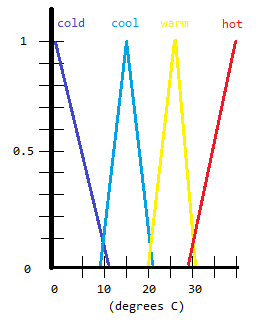
\includegraphics[width=\linewidth]{figure/mem_func.png}
        \caption{Example membership functions for the fuzzy variable temperature}
        \label{fig:mem_func}
    \end{subfigure}
    \newline
    \begin{subfigure}{.5\linewidth}
        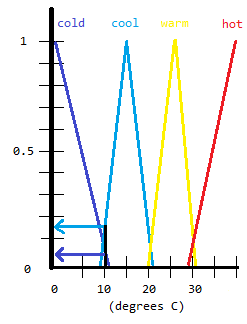
\includegraphics[width=\linewidth]{figure/fuzzification.png}
        \caption{Fuzzification of the crisp value 10 degrees to a fuzzy temperature value}
        \label{fig:fuzzification}
    \end{subfigure}
    \newline
    \begin{subfigure}{.5\linewidth}
        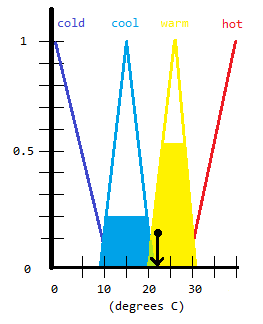
\includegraphics[width=\linewidth]{figure/defuzzification.png}
        \caption{Defuzzification of a fuzzy temperature value to 22 degrees.}
        \label{fig:defuzzification}
    \end{subfigure}
    \caption{Illustration of membership functions, fuzzification, and defuzzification process.}
    \label{fig:mem_fuzz_defuzz}
\end{figure}


\subsection{Fuzzification and Defuzzification}

In order to determine membership levels of fuzzy variables, membership functions exist for each linguistic term in the set to define a mapping of crisp values to amounts of membership in the fuzzy terms. Figure \ref{fig:mem_func} illustrates membership functions for the example temperature variable. It is often the case that membership functions overlap - if they did not, then values will only have membership in one term, which is essentially the same case as Boolean logic. The overlapping regions provide membership in multiple fuzzy terms. This is a critical distinction for fuzzy systems and allows a variable to express some uncertainty.

Membership functions can take any form or shape, but are commonly triangular or trapezoidal. More complex functions, such as Gaussian curves are also common candidates, especially when the problem domain is based on probability or statistics \cite{Ali2015ComparisonPerformance}. Much like the choice of activation functions in a neural network depends on the specific problem domain, the choice of membership functions may be driven by the domain to which the FIS is being applied.

Before a FIS can operate on input data, it must transform crisp input values into the fuzzy value space, i.e. map the values into the membership functions. The process of transforming crisp numeric values to the fuzzy values is referred to as \emph{fuzzification}. Similarly, the output of the FIS must be transformed back to crisp values for most applications. This reverse process, transforming a fuzzy value back to a crisp value, is called \emph{defuzzification}. Each of these processes are illustrated in \ref{fig:fuzzification} and \ref{fig:defuzzification}. 

Fuzzification is performed by evaluating each membership function for a variable on the crisp input. The resulting output of the membership function indicates the crisp value's level of membership in that particular variable. The crisp value is represented by the set of membership levels from all membership functions in the set, as shown in the earlier example.

Defuzzification rqeuires the combination of multiple membership levels to be reduced to a single crisp value. There are many methods for accomplishing this, and the selection of defuzzification method greatly impacts the results produced by the system. Common defuzzification methods include maximum membership, centroid, and bisector of area. The maximum membership method simply discards all but the highest membership term, and returns a scalar falling in that membership function (most commonly, mean-max membership is used to return the mean value of the range of the membership function). This means that for a given fuzzy variable, the same scalar will be returned in every case where that membership term is the maximum, regardless of what the membership level was. More complicated methods are based on the area under each membership function. For example, the centroid method returns the geometric centroid of the shape formed by the area under all of the membership functions, as illustrated in \ref{fig:defuzzification}. Similarly, the bisector of area method considers this shape and returns the point that bisects the area. These techniques are capable of returning a continuous range of crisp values, unlike the maximum membership method.

\subsection{Fuzzy Rules}

In this work, we use only Mamdani-type inference in which all variables are expressed as fuzzy sets. Rules in a Mamdani-style inference system are expressed in the form ``\emph{IF $X$ is $x_i$ and $Y$ is $y_j$ THEN $Z$ is $z_k$}'', where $X$, $Y$, and $Z$ are each fuzzy variables and $x_i$, $y_j$, and $z_k$ are terms belonging to the fuzzy sets. An example in a fuzzy system controlling a thermostat might be ``\emph{IF outsideTemp is cold and indoorTemp is low THEN heatSetting is high}.'' Rules may be conjunctive or disjunctive and may contain any number of operands in the rule.

During the evaluation of a rule, the level of membership of the input terms are considered to determine the strength of membership of the output. The Fuzzy `and' operator results in the minimum level of membership strength between the operand terms being passed to the output. By contrast, the fuzzy `or' operator results in the maximum level of membership strength between the two operands being passed to the output.

To illustrate the evaluation of rules, consider the previous example ``\emph{IF outsideTemp is cold and indoorTemp is low THEN heatSetting is high}.'' Let $outsideTemp['cold'] = .35$ and let $indoorTemp['low'] = .1$. The rule is evaluated as $heatSetting['high']=min(.35, .1)=.1$. The final output of the fuzzy system depends on the evaluation of the rest of the rules in the system and the defuzzification method used.

\section{Genetic Algorithms}
Genetic algorithms (GA) define a process for evolving high-quality solutions to a problem by mimicking the biological processes of natural selection and mutation \cite{holland1992genetic}. This process is often applied to large optimization problems as a means to approximate an optimal solution. Genetic algorithms begin with a set of sub-optimal solutions (the \emph{population}) and iterate through generations of offspring, evaluating generated child solutions against a fitness metric. By allowing the most fit solutions to combine and replicate at each generation, the final population will represent higher-quality solutions than the initial population.

 The structure of fuzzy systems, whose performance is dictated by a number of membership function parameters and rule sets, makes them natural candidates for optimization by a GA. There is much support in related literature for applying genetic algorithms to fuzzy systems \cite{seng1999tuning, karr1991applying, takagi1993neural}.

\subsection{Chromosome Encoding}
Candidate solutions in a genetic algorithm must be expressed as a set of properties (chromosomes) to facilitate the reproductive process. The method of encoding properties of a solution into chromosomes is highly dependent on the particular problem to which the GA is being applied. Popular choices include value encoding (e.g. binary, hexadecimal, real-valued) which directly encodes  values in an equation or system into different genes on the chromosome, permutation encoding which encodes the ordering of properties into the chromosome, or tree encoding which encodes tree or graph properties of a solution with a complex or graph-like structure (e.g. when using a GA to write an algorithm based on a graph of operations) \cite{kumar2013encoding}.

Since membership functions within a fuzzy system are easily expressed as sets of real values (e.g. for a triangular membership function, a triplet of real values $(x_1, x_2, x_3)$ define the function), the genes within the chromosomes representing fuzzy systems typically use simple value encoding. This allows the GA to evolve the solutions by altering the structure of membership functions within the system. Fuzzy systems are commonly initialized with rules based on intuition applied to the problem domain, but the mapping of crisp input values to fuzzy terms (i.e. the boundary of membership functions) is not always immediately clear. The GA approach provides support for finding appropriate boundaries for the terms. Additionally, GA optimization may find unnecessary terms by evolving a higher-quality solution in which one membership function completely envelopes another. In this case, the GA is capable of optimizing the structure of the system in addition to fine-tuning the membership parameters.

\subsection{Reproduction of Individuals}
The primary operations by which subsequent generations of a population are created by a GA are crossover and mutation. These genetic operations mimic biological reproduction and accomplish two goals: 1) the preservation of good features in the population (i.e. features which contribute high fitness), and 2) the introduction of random mutations (i.e. new features) into the population. 

Crossover is the process of selecting genes from each parent to build a chromosome for a child. Since only one parent may contribute a given gene, the method of mixing these genes can greatly impact the performance of the GA. Single-point crossover is performed by choosing a random point along the chromosome and including all genes from the first parent before the crossover point, and all genes from the second parent after the crossover point \cite{holland1992genetic}. This process generalizes to $k$-point crossover, where any number of points may be selected to alternate between genes from each parent. For real-valued gene encoding, different forms of blend crossover, where child genes are determined by some operation incorporating both parent values (such as averaging), may be used instead \cite{Eshelman1993Real-codedInterval-schemata}. However, the success of blend crossover depends on the level of correlation between output variables in the fitness function. Additional techniques may be required in non-separable cases \cite{Takahashi2001AAlgorithms, Buche2005AcceleratingModels}.

The crossover operation alone investigates solutions in new regions of the solution space. However, to fully mimic evolutionary processes and introduce some amount variability into the population, GA optimization also implements the mutation operation. After crossover is performed, mutation introduces new genetic information with some pre-determined probability. Mutations help to ensure that the population of individuals does not become entirely homogeneous and converge in a sub-optimal solution space \cite{holland1992genetic}. The implementation of mutation is dependent on the chromosomal structure. Real-valued genes may mutate by increasing or decreasing in value within some allowable range of the original value. Binary-encoded genes may mutate by simply flipping a bit in the target gene.

\subsection{Evaluating Fitness}
In each generation of the GA, the population is evaluated against a fitness metric to determine the most fit solutions. The fitness function represents the problem the GA is attempting to optimize. Fitness functions typically include accuracy, precision, recall, and/or cross-entropy, as would be expected in the training of any classifier. After evaluating each individual, the fitness may be used to inform which individuals are dropped from the population and how likely each individual is to reproduce. Techniques like roulette-wheel selection or tournament selection are popular choices that reward fit individuals with a higher probability of mating \cite{Zhong2005ComparisonAlgorithms}



\section{Optical Flow}
Several of the input features to our proposed fuzzy system are derived through optical flow. Optical flow is a category of algorithms that take two frames of video as input and provide an estimate of the motion vector for pixels in the frames, allowing for the approximation of the movement of objects in the video. For our activity recognition system, which is built on the theory that objects are a key indication of activities being performed, the movement of objects in the view of the actor is a key piece of information.

The motion estimation can be computed for every pixel in the input (\emph{dense}) or for a specific subset of pixels which have been identified as being important (\emph{sparse}). The motion estimates for pixels are computed by considering the linear displacement of corresponding pixels in the two frames as shown in Figure \ref{fig:optical_flow}. The optical flow algorithm provides an estimation of the vector $<dx, dy>$.

\begin{figure}
    \centering
    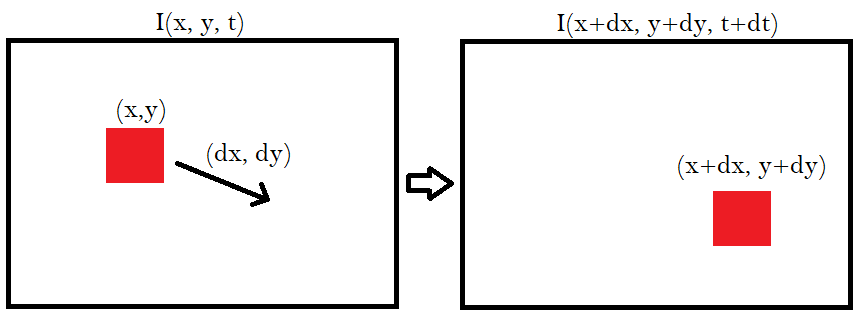
\includegraphics[width=\linewidth]{figure/optical_flow.png}
    \caption{The pixel specified in the first frame at time $t$, $I(x, y, t)$, translated by $(dx, dy)$ units and is located at $I(x+dx, y+dy, t+dt)$ in the next frame at time $t+dt$.}
    \label{fig:optical_flow}
\end{figure}

To compute optical flow, it is necessary to assume that pixels in the image $I(t)$ have equal intensity in the image $I(t+dt)$ for small values of $dt$. This is valid in practice because a small $dt$ represents a time difference where the appearance of the object and lighting conditions are unlikely to change drastically. Based on this, we can set the equation for each pixel in the two images as equal (known as the constant intensity assumption): $I(x, y, t)  = I(x+dx, y+dy, t+dt)$. This equation can be solved for the resulting motion vector using polynomial expansion, Taylor series approximation, and a variety of other methods \cite{Farneback2003Two-FrameOn, Horn1980DeterminingFlow, Lucas1981AnVision}.






\section{Convolutional Neural Networks}
In order for our proposed system to build an understanding of which objects are being interacted with, we rely partially on information about the actor's hands in relation to objects around them. We assert that most activities occur as interactions with objects in an environment, and hand position is a strong indicator (from a first-person perspective) of which objects are being interacted with. To this end, our system uses a convolutional neural network to determine hand location as input data to our FIS.

Neural networks are a set of machine learning techniques inspired by the structure of the human brain, where input data results in the stimulation of neurons, which in turn leads to information being passed on in a network of other neurons, which eventually lead to an intelligent output. Neural networks are composed of a variable number and type of layers of neurons (nodes) which are activated when the input they receive exceeds a threshold value. The activated neurons pass data through the layers of the network, performing various operations at each layer, until the output layer is reached. The weight given to each layer or neuron in determining the output is learned by the network through a training process. Neural networks can be used to classify and cluster data very efficiently, as they are very good at approximating complex functions.

Convolutional neural networks (CNN) are a special class of neural networks that contain convolutional and pooling layers. They are designed to learn spatial relationships of features in an input, which has lead to their popularity in applications such as computer vision and natural language processing \cite{Mane2020AApplications}. 

Unlike more traditional neural networks, where features are extracted from data prior to feeding inputs to the network, CNN's expect raw data and produce the features within the network. Features are extracted through convolution operations, which involve computing a kernel function as it slides over a provided input. The kernels functions are learned parameters of the CNN, and each kernel theoretically serves to extract a different type of feature. While the user of a CNN does not specify the features and kernels, visualizing the trained kernels on images often reveals that features learn to extract similar information to traditional features, such as color, edge, and texture descriptors.

In addition to convolution layers, pooling layers are used within the network to reduce the dimension of features extracted in later layers. Pooling is an operation that condenses information within a neighborhood of each data point, through operations like averaging or taking the maximum value. The result is that convolutional layers deeper in the network have lower dimensionality, and therefore represent more abstract features about the input than earlier layers \cite{Zeiler2014VisualizingNetworks}. This allows CNN architectures to perform robust detections on data that may require knowledge of features that have varying spatial or temporal correlations by extracting features at multiple resolutions.

\subsection{MobileNet}
In the field of CNN's, there are several commonly used and notable architectures, including AlexNet \cite{Krizhevsky2012ImagenetNetworks}, ResNet \cite{He2016DeepRecognition}, and VGGNets \cite{Simonyan2014VeryRecognition} among others \cite{Li2021AProspects}. These models have gained popularity for solving different challenges within CNN's, such as optimizing network size or speed, efficiency of training, or overall performance in specific types of tasks. The hand detection network included in our proposed solution uses the MobileNetV2 \cite{Sandler2018Mobilenetv2:Bottlenecks} architecture. This network is specifically designed for low-resource applications, such as mobile or edge computing while retaining accuracy competitive with larger networks. While our stated goals for this work do not include performance optimizations, the MobileNetV2 model provides a convenient and accessible solution for an activity recognition system that may someday have such constraints.

Our MobileNetV2 model uses a version of the Single Shot Detector (SSD) \cite{Liu2016Ssd:Detector}, specifically the Feature Pyramid Network (FPN) \cite{Lin2017FeatureDetection}. While traditional object detection models approach detection by proposing bounding boxes, then resampling features for each box, and finally applying a classifier to each box, the SSD method eliminates bounding box proposal and the feature resampling steps by producing predictions of different scales using features maps of different scales, computing the information in a single pass through the network. The accuracy of SSD is shown to be more accurate than previous state-of-the-art while being much faster.


%================================================
\chapter{Experiments and Results}
%================================================

This chapter describes the experimental methods and results achieved in the process of resolving the research questions posed earlier. 

%================================================
\section{Gait Speed Comparison from Wearable Camera and Accelerometer Vest in Structured and Semi-Structured Environments}
%================================================
To address our first research question \emph{(Can wearable sensors be used to unobtrusively monitor activities of subjects in a semi-structured environment?)}, we limited the scope of activities to a single activity - gait. By considering only a single activity, much of the complexity of the problem was eliminated, instead focusing on determining the ability of various sensors to describe the parameters of the activity in semi-structured environments, i.e. home-like, controlled, indoor setting without the visual noise of environmental motion found in public settings. While the focus was on a single activity and the primary concern was validating the use of wearable sensors - in particular, vision-based sensors - for activity recognition, this work still presented potential for meaningful outcomes due to the strong correlations of gait quality to a number of medical concerns. \emph{This work was described in \cite{Schneider2019ComparisonEnvironments}. A modified version is provided below in this section.}

\subsection{Overview}

Gait analysis is an area of research that has seen an increasing focus due to its applicability to a wide range of age-related health issues which may impact the growing elderly population \cite{Ortman2014AnStates}. For example, Beauchet et. al found evidence that dementia can be predicted by poor gait performance \cite{Beauchet2016PoorMeta-Analysis}. Similarly, Valkanova and Ebmeier show that evidence strongly supports a relationship between gait and impairment of cognitive functions in patients with mild cognitive impairment and Alzheimer's disease \cite{Valkanova2017WhatEvidence}. These findings illustrate the potential of using gait analysis in detecting symptoms of age-related illnesses.

While many objectively quantifiable gait parameters could be used for effective decision support and automated monitoring, the simple measure of \textit{gait speed} has shown to be an accurate predictor of mobility, health, and even mortality \cite{Afilalo2010GaitSurgery, Viccaro2011GaitForce, Fitzpatrick2007AssociationsPersons}. Gait speed is thus a critical parameter for evaluating the utility of candidate gait analysis systems. Therefore, the goal of this study was to determine the feasibility of using our wearable system, comprising an affordable and non-invasive wearable camera and computer-vision based processing methods, to classify the gait speed of healthy individuals. Samples of gait were collected at three self-determined over-ground walking speeds (slow, medium, fast). Since accelerometer-based methods have been successfully used to quantify gait, we deployed an accelerometer near the subject's right hip for the purpose of providing a direct point of comparison for our system to a more widely-used device. We also compared the capabilities of both devices to a research-grade optical motion capture system which represents the ``gold standard'' for gait analysis. The comparison to both another previously studied wearable system and a high-precision standard provides validation for using our single-camera system for gait analysis tasks.

Expensive laboratory-based gait analysis systems can provide extremely robust quantification of human gait and locomotion. For example, highly precise three-dimensional motion capture systems have recently been used to study detailed gait features across age groups in healthy individuals \cite{Chien2015TheIndividuals} as well as individuals with Parkinson's disease \cite{Corona2016QuantitativeDisease} and Alzheimer's disease \cite{Rucco2017Spatio-temporalCapture}. While these systems can often provide an in-depth description of gait, they are not feasible for the use-case of continuous monitoring due to their size, complexity, and cost. Continuous monitoring of patients in their natural environments during everyday activity provides a more constant and natural sampling of gait activity, enabling the detection of changes in performance over time. Additionally, user-friendly and lower cost pervasive health monitoring systems reduce the burden on patients to make trips to a physician's office, which may be especially cumbersome for the elderly.

Recent work focused on providing convenient, in-home solutions for activity recognition, eliminating the need for a laboratory setup. Video-based methods may offer inexpensive solutions with performance similar to more sophisticated motion capture systems or floor sensors \cite{Wang2013TowardAdults}, but suffer from obstructed line-of-sight within the home environment. Audio-based systems have also been used to analyze gait in indoor environments \cite{Geiger2013Gait-basedFeatures, Altaf2015AcousticSounds}. While both audio- and video-based systems have shown promise, their use is limited to a specific preconfigured location. To overcome these issues, gait analysis is also being performed with wearable devices, such as smart watches \cite{Suh2016Kalman-Filter-BasedSmart-Watch}, shoe-based wearable sensors \cite{Mariani2013On-shoeDisease}, and wearable accelerometers \cite{Fortune2014ValidityVelocities, Hartmann2009ConcurrentAdults, DelDin2016ValidationUse, Chung2012GaitAccelerometer}. By instrumenting the subject instead of the environment, the systems become portable and problems such as line-of-sight obstruction can be avoided. While these solutions provide promising results for gait analysis, they tend to be either still too complicated for in-home use (e.g., due to the number of components), or incapable of matching the level of precision and capturing gait performance as comprehensively as  laboratory-grade motion analysis systems. Thus, there are trade-offs between accuracy and cost for laboratory-grade motion analysis systems and in-home wearable systems for gait analysis.

Our system used a single head-worn camera to collect first-person video. Using computer vision techniques, we were able to extract optical flow output from the video that mimics the ability of a low-resolution accelerometer to register movement parameters \cite{Schneider2017PreliminaryProcessing}. A benefit of a vision-based sensor such as this is that the video data can provide additional context to the in-home monitoring scenario. For instance, if an unexpected event occurs with respect to gait speed, the monitoring system could notify additional automated or manual review processes to analyze the specific related video segment and determine whether the event was a clinically significant event, such as a fall, or simply an abrupt stop. It may also be possible to analyze the coarse direction of the subject's visual attention while walking and to identify objects that are being interacted with - a key capability that is exploited in the FIS described later in this document - or other factors that may impact gait performance. Methods based entirely on accelerometer or pressure sensors are unable to explain variations or interruptions that are seen in daily gait activities and would not be able to inform further analysis processes. While vision-based in-home monitoring systems may raise privacy concerns by recording subjects and others in their home, automated methods of processing the video upon recording would eliminate the need to store the raw video, mitigating the privacy risk. The storage or transmission of computed motion-based features removes all identifying information as these features are essentially equivalent to those recorded by inertial sensors, which do not raise the same concerns.

Our previous work based on the use of a wearable camera (and accelerometer for comparison as a well-established device) involved collecting data from subjects on a treadmill \cite{Schneider2017}. However, limiting the data collection to occur on a treadmill was an artificial constraint, especially for the in-home use-case being described. In this experiment, we remove the limitation and also investigate the impact of changing this aspect of the experimental design to incorporate semi-structured, natural, over-the-ground gait sequences from nineteen participants.

\subsection{Data Collection}

\begin{figure}[!t]
\centering
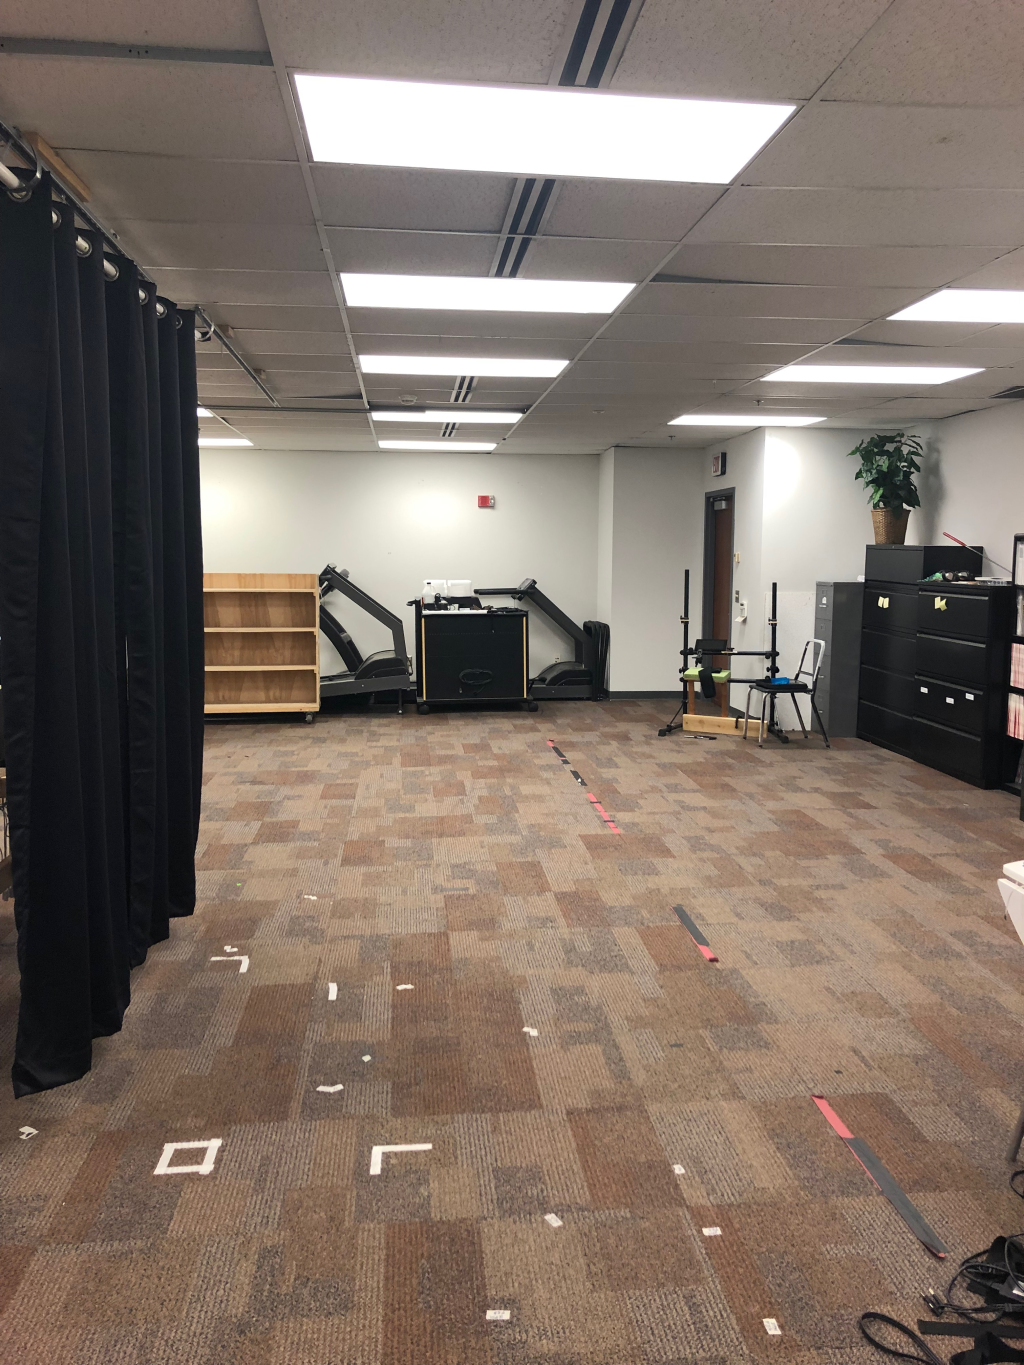
\includegraphics[width=1.8 in]{figure/MoCapRoom}
\caption{The motion capture laboratory in which data was collected from participants}
\label{fig_mocap}
\end{figure}

\begin{figure}[!t]
\centering
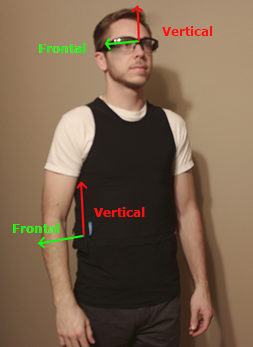
\includegraphics[width=1.8 in]{figure/sensorAlign}
\caption{Placement of Sensors on Subject and Alignment of Axes Between Sensors}
\label{fig_axes}
\end{figure}

Accelerometer, motion capture, and first-person video data were collected from nineteen participants as they walked over ground six times, covering a distance of four meters, in a large motion capture laboratory. The space was free from any physical obstructions such as furniture or walls (Figure \ref{fig_mocap}). The participants were healthy college students ranging from 18 - 21 years old. Ten of the participants were male and the remaining nine were female. Participants were instructed to walk at three self-determined speeds: slow, medium, and fast. Categorical speeds were used for multiple reasons. First, as participants were walking over the ground, and not on a treadmill, it would have been difficult to adequately control gait speed. Second, the time series data from inertial sensors and the processed video features indicated the frequency of each subject's gait, which directly correlates to gait speed. Estimating the continuous gait speed requires knowledge of the exact stride length of a subject. Categorical gait speed was thus more appropriate as slow, medium, and fast gaits naturally correspond to an increasing step frequency regardless of stride length or distance covered.

Each subject wore two commercial devices during data collection (see Figure \ref{fig_axes}). The Pivothead SMART Architect Edition glasses \cite{Pivothead2017Pivothead} were used to record video of the activity in high-defintion resolution (1920 x 1080) at 30 frames per second. The device is a pair of eyeglasses with a camera located in the center of the glasses, above the nasal bridge, aimed directly forward. The glasses are nearly indistinguishable in shape and weight from a normal pair of glasses, providing a comfortable and natural sensor that is easily integrated into daily routine with no encumbrance or health risks to the wearer. The Hexoskin smart shirt \cite{CarreTechnologies2017HexoskinShirts, Banerjee2017ValidatingManagement} was also worn, providing tri-axial accelerometer readings at 64 Hz (data from the remaining sensors in the Hexoskin shirt were not analyzed for this study). The accelerometer was located near the right hip on the torso of the subject inside a pocket of the shirt. Gait data were also recorded with a 20-camera Motion Analysis Corporation Kestrel motion-capture system at a sampling rate of 120 Hz, and motion data were processed using Cortex v. 6.2 software (Motion Analysis Corp., Santa Cruz, CA). Each participant was instrumented with motion capture markers according to the Cleveland Clinic marker set. This model includes markers tracking the position of the feet, legs, trunk, arms, and head. While the position of each marker was recorded, our analysis focused on the head marker (for comparison to the head-worn glasses results) and estimates of whole-body center of mass derived from the global marker set using a whole-body mass model calculated from Zatsiorsky-Seluyanov's body segment inertia parameters \cite{deLeva1996AdjustmentsParameters}. Each of the three systems independently and simultaneously recorded the gait sequences that were performed.

The Pivothead glasses were purchased for \$300 USD and the Hexoskin vest and device may be purchased together for \$499 USD, making them easily available to consumers. While the exact price of the motion capture system is not immediately available and will vary based on configuration, the cost of the 20-camera system is roughly \$100,000 USD. A minimal set of four lower-precision cameras could be obtained for less than \$10,000 USD. Even considering the lower-cost motion capture option, the consumer-grade devices have the advantage of being easy to use, while the motion capture system requires an expert user, calibration of the system, and extensive instrumentation of the subject. While the motion capture system presents an excellent means for collecting our high-precision truth data, the cost and complexity dictate that the motion capture system will only be feasible in a controlled clinical laboratory, and not for continuous, in-home monitoring. While we did not investigate real-time processing, the computational requirements for data from the single camera and inertial sensor would also be much lower than the 20-camera system.

\begin{figure*}
\centering
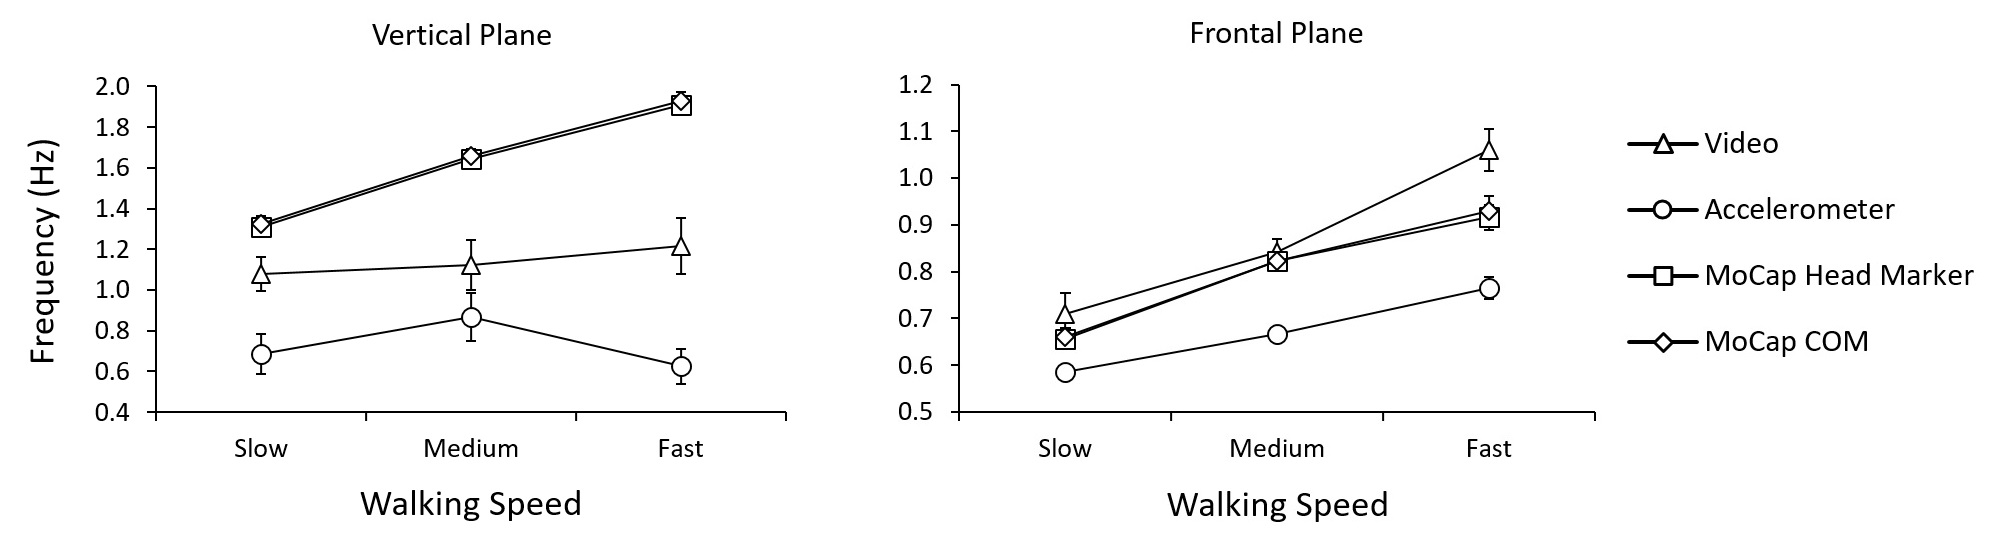
\includegraphics[width=7in]{figure/meanplots}
\caption{Mean Plots with Standard Error Bars for Recorded Features By Gait Speed}
\label{fig_meanPlots}
\end{figure*}

\subsection{Signal Processing}
The intent of incorporating the glasses-style camera into the experiment was to use the collected video to describe the subject's head motion in two dimensions (the frontal and vertical planes) throughout the gait sequence. Since the camera faced directly forward from the participant, the frontal and vertical axes in physical space (relative to the participant) correspond to the x- and y-axes of the recorded video. While the camera device collected less data and operated at a lower sampling rate and spatial resolution than a highly accurate 3-D motion capture system, the device was extremely portable, affordable, and simple to operate. However, the lower-fidelity visual data produced by the camera required careful processing in order to extrapolate information about the movement of the subject who is not in the view of the camera. The Lucas-Kanade optical flow technique was applied to the collected video samples in order to estimate participant motion from the videos \cite{Lucas1981AnVision}. This method produced a displacement vector for a series of significant keypoints within a given video frame. An average vector was computed from all keypoint vectors per frame, resulting in a single two-dimensional vector which represented the overall displacement of the participant in each frame of video. This approach was previously validated against other possible computer vision techniques and was found to provide the most accurate representation of the actual displacement between frames \cite{Schneider2017PreliminaryProcessing}.

The two-dimensional (frontal, vertical) components of the optical flow displacement vectors were considered over time to generate two separate sets of time series data. Three-axis time series data were also collected from the body-worn accelerometer, and head and center of mass data (each in three dimensions) from the motion-capture system were also analyzed. The time series data were manually separated into segments collected during each of the six trial walks performed by each participant. The collected data were manually segmented into six trial walks by examining the video and audio, and then recording the start and stop times of each gait segment within the video. None of the systems directly provided a determination of when a gait sequence occurred, though it would be feasible to automate this detection based on the collected features and the video data. For this initial work, such a system was not developed as the focus remained on considering only the data recorded during known gait activities. Motion-capture data were filtered in Cortex using a 4th-order low-pass Butterworth filter with a cut-off frequency of 6 Hz, which is the default setting for the low-pass filter in Cortex. Cut-off frequencies in motor control research generally range from 6 to 10 Hz, depending on the behavior being observed. Given that the observed behavior was walking, 6 Hz was much higher than the frequencies of interest and only filtered out sensor noise.

Because the wearable devices were commercial devices which operated independently of each other, it was not possible to guarantee perfect synchronization of the data collection across devices. This precluded any direct comparison of the raw time series data from each of the sensing devices, since errors in synchronization of the collected data would negatively impact any calculations. However, it is not necessary to directly compare the time series data - gait speed alone has been shown in clinical applications to be a predictor of cognitive disorders such as dementia \cite{Bramell-Risberg2005LowerControls}. To overcome the limitation on direct comparison between the time series data from each device, we moved data out of the time domain and instead derived frequency-based features in the following manner. 

A periodogram calculation was applied over the entirety of each walk segment for each channel of data being considered. As shown in \cite{Schneider2017PreliminaryProcessing}, the periodogram transformation can be used to identify main frequencies that occur in each time series. We identified for each time series the frequency with the highest amplitude from the computed periodogram to serve as our gait metric. While the periodogram provides an analysis of constant gait speed in \cite{Schneider2017PreliminaryProcessing} and a successful indication of gait speed in temporally short gait sequences collected for this study, longer gait sequences containing changes in gait speed may be better analyzed with methods that consider time locality, such as a spectrogram. For this study we have assumed that gait speed was constant in each gait segment.

\subsection{Statistical Analysis}
The goal of this work was to determine the feasibility of classifying gait samples categorically by their speed with a specific interest in the performance of the video-based wearable system. We determined whether the collected video-based features were impacted by gait speed in a manner similar to the features from more traditional gait analysis devices. We used analysis of variance (ANOVA) to determine whether our gait metric was significantly impacted by gait speed. Separate ANOVAs were conducted for each plane of motion for each gait measurement system. Data were screened for outliers ($\pm$ 2.5 standard deviations from the median) prior to analysis; 6 trials were identified as outliers, all for the motion capture system in the sagittal plane and likely resulted from obstruction of one or more markers from the motion capture cameras' view. Violations of the sphericity assumption were resolved by correcting the degrees of freedom of the statistical test using the Greenhouse-Geisser method.

\subsection{Results}
ANOVA on the frequency-based gait metric derived from the eyeglass camera data revealed no significant differences across gait speed conditions in the vertical plane ($p= .55$, $\eta^2_p = .04$). However, in the frontal plane, there was a significant effect of gait speed, $F(1.49, 22.39) = 36.0$, $p < .001$, $\eta^2_p = .71$.Pairwise post-hoc comparisons revealed significant differences among all three speed conditions (fast vs. medium: Cohen's $d= 1.96$; fast vs. slow: $d= 1.76$; medium vs. slow: $d= 0.75$; all $p< .05$). This indicated that using the frontal plane data ($u$ for the glasses), the sensor was able to distinguish between gait speeds across the three categories. 
 
As was the case with the camera data, the accelerometer data did not discriminate gait speed conditions in the vertical plane ($p= .26$, $\eta^2_p = .09$). There was a significant effect of gait speed in the frontal plane, $F(1.6, 23.98) = 11.43$, $p < .001$, $\eta^2_p = .43$. Post-hoc tests again identified significant differences among all three speed conditions (fast vs. medium: $d = 0.69$; fast vs. slow: $d= 0.99$; medium vs. slow: $d= 0.68$; all $p < .05$).
 
For the motion capture system, we first considered data from the head marker. A significant effect of gait speed condition was observed in the vertical plane, $F(1.41, 21.1) = 160.2$, $p < .001$, $\eta^2_p = .91$. All three speed conditions were found to differ significantly according to post-hoc tests (fast vs. medium: $d= 2.78$; fast vs. slow: $d= 3.51$; medium vs. slow: $d= 2.65$; all $p< .001$). A significant effect was also observed in the frontal plane, $F(1.25, 18.79) = 66.97$, $p < .001$, $\eta^2_p = .82$. All three speed conditions were found to differ significantly according to post-hoc tests(fast vs. medium: $d= 0.78$; fast vs. slow: $d= 3.11$; medium vs. slow: $d= 2.81$; all $p< .01$).
 
For the center of mass displacements calculated from the motion capture data, ANOVA revealed significant effects of gait speed in each plane of motion. In the vertical plane [$F(1.37,20.04) = 175$, $p < .001$, $\eta^2_p = .92$], post-hoc tests revealed significant differences among all conditions (fast vs. medium: $d= 3.17$; fast vs. slow: $d= 3.64$; medium vs. slow: $d= 2.69$; all $p< .001$). Likewise, for the frontal plane [$F(1.19,17.88) = 68.52$, $p< .001$, $\eta^2_p = .82$], all pair-wise post-hoc comparisons were significant (fast vs. medium: $d= 1.06$; fast vs. slow: $d= 2.3$; medium vs. slow: $d= 3.81$; all $p< .05$).

\subsection{Conclusion}
In this particular experiment, we evaluated the performance of a gait analysis system which used only a wearable camera to collect two-dimensional, first-person video. Optical flow and frequency domain analysis were used to generate a dataset from video, and this dataset was then compared to data collected with a wearable tri-axial accelerometer and a 20-camera motion capture system. This was a crucial step to validate the use of a single-camera wearable system against the vest device and the gold standard motion capture system. While both of the latter devices (the accelerometer and motion capture systems) have seen more use in the domain of wearable gait analysis than the wearable camera, the camera-based system has several advantages including cost, simplicity, and the ability to analyze the visual scene to provide context for the gait analysis data. Although the motion-capture system provided superior discrimination of gait speed in all planes of motion, as expected, the eyeglass-based camera system nonetheless discriminated gait speed significantly and outperformed the vest-based accelerometer system. This suggests considerable promise for its use in unobtrusive activity monitoring in a semi-structured environment.

The results of this experiment demonstrated the ability to detect a clinically significant factor of gait performance using only a wearable camera. Additionally, the experimental setup validated that such a device did not interfere or alter the method of performing the activity. This was an essential outcome for positively concluding that the wearable vision-based device is both convenient and useful for detecting activities in an unstructured, in-home environment.

%================================================
\section{Describing Object-centric Activities using Fuzzy Methods}
%================================================
To address our remaining research questions, (\emph{RQ 2: Can features extracted from first-person videos recorded in subjects’ homes be used to categorize different interactions with objects?}), and \emph{RQ 3: Can the activity identification system a) accurately describe activities and b) handle uncertainty in the results better than current state-of-the-art methods?}, we removed the limited scope of a single activity from the previous experiment and brought forward the use of a wearable camera and some of the input features from the first-person video. After validating the wearable device, the remaining experimentation focused on identifying the occurrence of activities based on the users' interactions with objects.

\subsection{Overview}
Recognizing and understanding human activities occurring in video is an important enabling technology to a variety of computationally intelligent systems. The spectrum of all possible human activities is extremely broad, with great variance in both the temporal and spatial aspects of activities. These activities can be placed on a scale of increasing complexity, with simple (or \textit{atomic}) actions occurring on the low end of the scale, i.e. activities occurring for a short period of time or with a limited number of movements, and highly complex or composite activities occurring on the high end if the scale, i.e. activities which contain other simpler activities as sub-components occurring in some order over a longer period of time. Identifying the exact point in time when an atomic activity (e.g. picking up a spoon) turns into a complex activity (e.g. making a cup of coffee) with any amount of objective precision is nearly impossible. This dilemma illustrates an inherent amount of fuzziness in the domain of activity recognition. That is, an activity may be described in multiple ways, at multiple levels of specificity, with each overlapping description retaining full accuracy.

In this experiment, we sought to address the challenge of handling the natural fuzziness in activity recognition that arises from the overlapping boundaries between activities and their definitions. We used fuzzy logic to discover object-based activities in first-person video of daily activities in kitchen environments. Using a variety of extracted features and object annotations from the video, the system was able to describe a diverse set of activities and provide information on the nature of activities without requiring extensive training. We sought to describe activities more completely and reliably than current uninterpretable or black box methods. Such a system can be used to detect activities more effectively in an in-home setting with applications such as aging in place for older adults, or other rehabilitation applications. A description of a preliminary version of this system was provided in \cite{Schneider2021BridgingVideo}.

Traditional work in the field of first-person activity recognition is often focused on exploiting information about objects in the scene in order to classify activities being performed \cite{Nakatani2019, McCandless2013, Pirsiavash2012, Sudhakaran2018, Wang2018}. The use of object-based activity models has shown promise, since many of the activities that people perform in their homes on a daily basis are largely based on the use of some object. However, visual noise, such as occlusion of the objects, negatively affects the object recognition accuracy, and thus greatly dampens the accuracy of the activity recognition framework as it relies heavily on the identification of objects the human is interacting with. Related works have shown that this noise can be reasonably handled with current object recognition techniques. Deep learning and convolutional networks can be very robust in classifying objects which are partially occluded or may have changing appearance based on the state of the object or the angle of the view. \cite{Pirsiavash2012} takes advantage of visual differences in the appearance of objects over time to determine whether an interaction is occurring.

Many of the more recent works in this field of study have abandoned traditional video features in favor of deep learning techniques to identify activities occurring in first-person video.   \cite{Li} features a recurrent convolutional neural network (R-CNN) trained on RGB images, optical flow, and gaze annotations. Similarly, \cite{Ryoo2015} describes the use of CNN features in a pooled time series representation in combination with a non-linear SVM to identify activities. \cite{Purwanto2017} applies the Hilbert-Huang transform to CNN features and uses an SVM classifier to classify activities. CNN-based techniques are favored for their ability to discover useful features in images and video, but the networks require extensive training. Due to the amount of training required, the set of activities classified by each of these CNN-based systems tends to be fixed and small relative to the complete set of daily human activities.

While the deep learning techniques may perform well for a small set of actions when trained against extensive annotated datasets, the requirement of massive amounts of labeled data is a huge limitation in the utility of such methods for activity detection and recognition. Given the multitude of activities that may occur on a daily basis, it is not simple to build a training dataset for a system that recognizes a complete set of these activities. Additionally, when these deep learning methods fail to recognize an activity, there is often no meaningful output - the deep learning techniques operate as a “black box” and the correlation between features and the output of the system is not usually well understood outside of that box. Consequently, the identification of an activity has a binary outcome, and when the classification is incorrect, the system provides little or no useful information.

We seek to remove these limitations through our use of fuzzy logic. In building a FIS to classify activities, extra work must be done to extract and understand video features and their correlation to activities recognized by the system, but the understanding of these features and parameters provides insight into the type of activity being performed even if the actual name of the activity is unknown. That is, a fuzzy system can provide a result which indicates aspects of the occurring activity without the need to positively identify the activity, incorporating uncertainty that is extremely useful for reliable performance in dynamic environments \cite{Anderson2009}. For many purposes of activity detection, including in-home monitoring of elderly \cite{Banerjee2015, Anderson2009a} and medical patients, human-machine interaction, or life-logging, the fuzzy information may be informative where artificial intelligence techniques produce no useful information.

We took inspiration from existing methods and extracted both motion- and object-based features from a set of first-person videos. Following is a description of a fuzzy inference system that uses these features to classify activities occurring in these videos. To our knowledge, the application of fuzzy methods to egocentric activity classification is a novel approach.

Our goal was to create a fuzzy inference system that classifies a set of activities being performed by the subject of first person videos. We acknowledge that the recognition of an activity is not always a binary decision given the relationships between various atomic and complex activities. For example, multiple atomic activities may occur simultaneously as part of a more complex activity. For this reason, we demonstrate a fuzzy system of activity recognition which provides a depiction of multiple aspects of the activities being performed. A simple diagram of the system is provided in Figure \ref{diagram}.

\begin{figure}[t]
\centerline{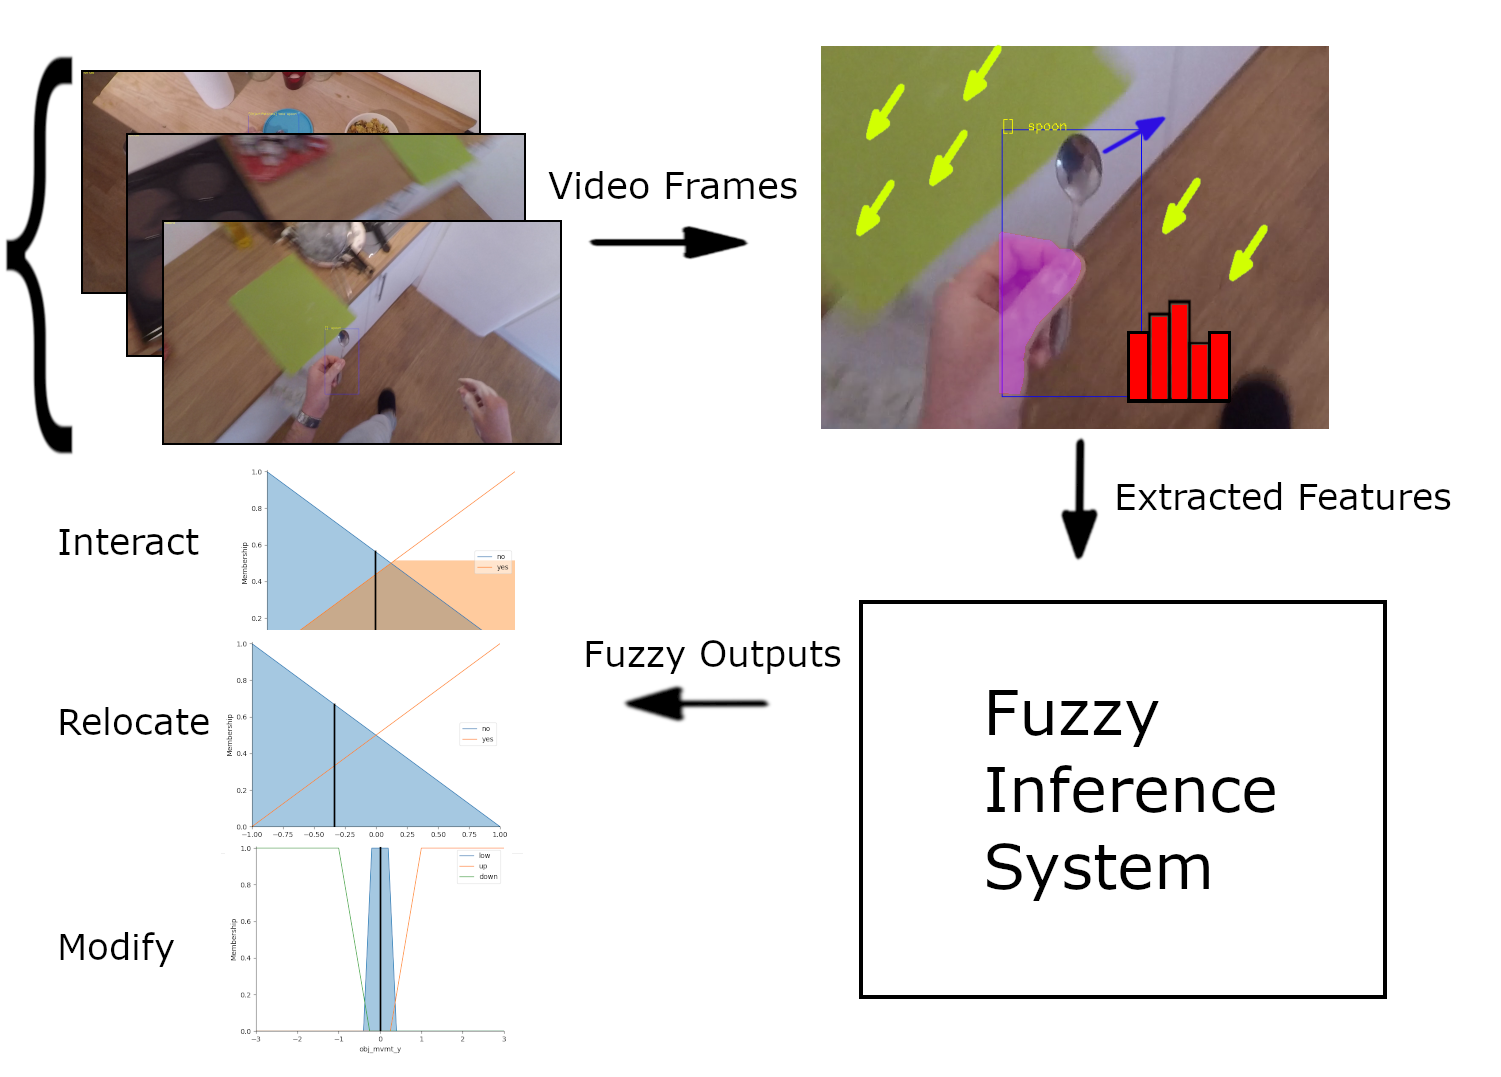
\includegraphics[width=.9\linewidth]{figure/diagram.png}}
\caption{Illustration of our system. Features such as optical flow motion vectors and color histograms are extracted from video frames and passed to the fuzzy inference system, which calculates fuzzy membership in three outputs based on a series of rules within the system.}
\label{diagram}
\end{figure}

\subsection{Dataset}
In previous experiments, the target environment for activity detection was either structured or semi-structured. This control of environmental variation lessened the number of factors which impacted the results, but was not realistic for a system that is capable of daily, in-home use, which is a key piece of research question 2. For this experiment, the environmental control was completed lifted to include video that was recorded in a true home environment. To avoid the complication of collected a custom dataset for our work, we surveyed existing datasets to find one that provided appropriate videos and labeled truth.

For this work, we used the EPIC-KITCHENS 2018 dataset \cite{Damen2018ScalingDataset}. This dataset contains unscripted first-person videos of subjects performing daily activities such as cooking, washing dishes, and cleaning in their kitchens. The dataset provides annotations of objects of interest, as well as annotation of the action involving the objects. The action annotations provided with the dataset comprise over 100 different verbs and highlight the amount of variability found in daily in-home actions in just a single room. The dataset is unscripted, which was an important feature to ensure that the data truly represents the intended use-case for our research questions.

While the intent of the proposed FIS system is to describe a potentially unconstrained set of daily activities, it would not have been feasible to simply build the FIS to output a single classification out of hundreds of activities. The FIS was instead built to output fuzzy descriptive features of the activities, classifying them into multiple categories of intent. While this meant that the FIS was not producing a specific activity label, this classification method provides insight into what is actually happening in the activity, which can provide description of even activities that the system was not trained on, alleviating the limitation that many classifiers have with only performing on a specific set of activities.

The output of the FIS focuses on three types of object-actions: interaction, modification, and relocation. Modification intent was defined as an action that intends to change the appearance or structure of an object. Relocation intent was defined as an action which intended to move an object in space. Other interactions which did not seek to perform modification or relocation were simply labeled 'interaction'. A categorization of main intent was determined for each annotated truth action in the dataset and appended to the annotations. While our expectation was that actions will have some membership in more than one output category, each action was given a single label for the most likely intent. For example, the action `pick up' provided in the original annotations received an intent label of `relocation', the `cut' action was labeled as modification, and the `wash' action was labeled as `interaction'. The additional intent labels were determined per action class and not per individual instance of the action, i.e. a given verb was considered to always have the same intent.

\subsection{Features}
As previously mentioned, building an FIS to analyze actions in video required manual feature selection and extraction. We build our fuzzy inference system around a set of features that are extracted from the three-channel first-person videos described in the prior section. The recognition of activities via the fuzzy rules in our system is predicated largely on the identification of objects in the video. The presence and motion of individual objects in the scene and their relation to the subject are critical inputs to the fuzzy inference system. The set of input features was built intuitively from this observation.

Table \ref{videoFeatures} lists each of the video features which are used as inputs to the fuzzy inference system.

\begin{table}
\caption{Video Features}
\begin{center}
\begin{tabular}{p{5cm}p{7cm}}
\hline \\
\textbf{\textit{Feature}}&\textbf{\textit{Description}} \\
\hline
\hline \\
\textit{Object bounding box} & the location of a rectangular bounding box around each identified object in the video \\ \\
\textit{Object label} & the name of each identified object \\ \\
\textit{Frame optical flow} & the mean, 2-dimensional optical flow vector in the video frame computed between frames $t_0$ and $t_1$\\ \\
\textit{Object optical flow} & the mean, 2-dimensional optical flow vector in the video frame computed between frames $t_0$ and $t_1$ within the bounding box of an object \\ \\
\textit{Color histogram difference} & the distance metric of the color histogram within the bounding box of an object in frames $t_0$ and $t_1$ \\ \\
\textit{Hand intersection} & the ratio of pixels within the bounding box of an object that are identified as belonging to a hand \\ \\
\textit{Keypoint similarity} & a ratio of matching keypoints to all keypoints detected on an object over a time step \\ \\
\textit{Object centrality} & a measure of how near the object is to the center of the visual window. \\
\hline
\end{tabular}
\label{videoFeatures}
\end{center}
\end{table}

\subsubsection{Object Features}
The fuzzy system was provided with a rectangular bounding box for each object in the scene. The bounding box for each candidate object was read from the dataset annotations, i.e. no object detection was implemented for this work. The annotations include bounding boxes at all times when objects involved in actions as well as some cases when they are not in use. The bounding box information was used to isolate the object for calculating several of the object-descriptive features discussed below.

\paragraph{Centrality}
The one feature which is computed directly from the bounding box is the centrality metric. An analysis of action locations in a subset of the training data revealed that the distribution of actions tends toward the center of the camera's perspective. This result is expected, since the center of the video represents the center of a subject's field of view, and thus a likely location for the initiation of an action. \ref{action_locations} illustrates the distribution of actions in this training data. Centrality of each object is computed by the two-dimensional distance from the center of the video, $(v_x, v_y)$ to the center of the bounding box $(b_x, b_y)$, subtracted from 1 to achieve high centrality when the distance is low and low centrality when the distance is high: \\
\begin{equation}
    centrality = 1 - \sqrt{(v_x - b_x)^2 + (v_y - b_y)^2}
\end{equation}

\begin{figure}[t]
\centerline{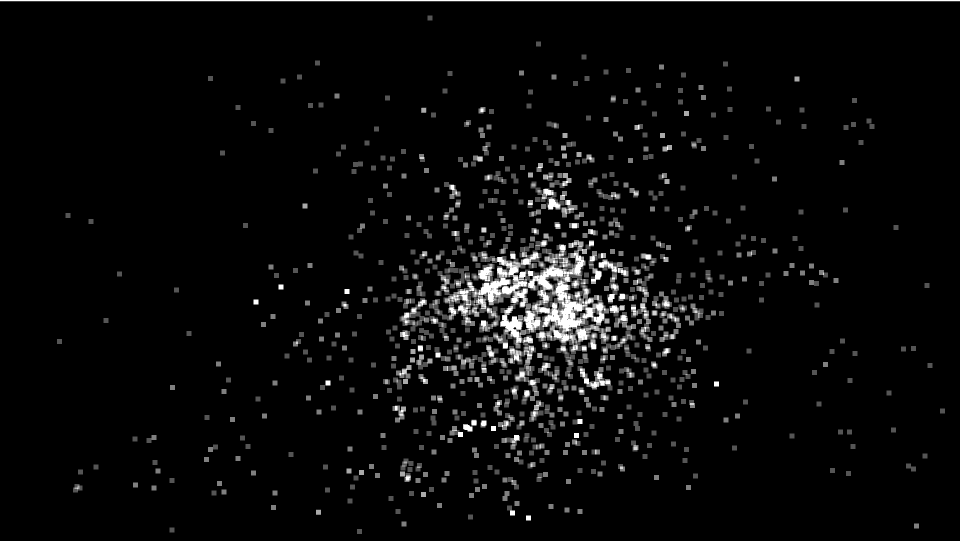
\includegraphics[width=.9\linewidth]{figure/action_locations.png}}
\caption{Illustration of the distribution of action locations within the training data.}
\label{action_locations}
\end{figure}

\paragraph{Object Appearance}
The change in appearance of an object over time is another logical feature that may inform whether the object is being interacted with, and whether the object is being modified or manipulated in some way. Previous work has been done on exploiting the change in appearance of objects to indicate the occurrence of activities \cite{Pirsiavash2012}. Two types of features were implemented to provide insight into different types of change to the object. 

Change in color is one of the simplest ways to perceive changes in an image. Features derived from the distribution of colors within a region of an image have long been used in literature to provide a measure of object similarity for use in object comparison and tracking applications \cite{Swain1991ColorIndexing, Chang1999ObjectHistograms, Wang2007AdaptiveFilter, Zivkovic2004AnTracking}. While more complex methods are required for complex tasks such as tracking objects, our system implemented a color histogram difference feature. This feature was useful for approximating the amount of change in an object's appearance over a time period. The color values were split into eight bins in each channel of the image to build the histogram, and the histogram was computed for all pixels within the object bounding box for two different frames. The final difference feature provided to the FIS was given by applying the intersection distance metric between the two histograms.

While color information is a simple indicator of change in object appearance over time, it is frequently the case that an object may be modified in a way that does not change the color of the object. In these situations, the color histogram feature alone was unable to inform the FIS on whether the object had been modified. To improve the robustness of the overall indication of object change, keypoint-based features were also introduced to the FIS. Keypoint detectors are responsible for choosing points within an image that are most meaningful to the image. Most often keypoint detectors identify points like corners, edges, or other complex shapes or textures that are integral to the appearance of the image. These keypoints can be compared across images to perform object recognition \cite{Oji2012AnKeypoints, Nowak2014SpatialRetrieval}. 

In the case of our FIS, the keypoints were detected within an object bounding box and matched between two different frames, and the ratio of matching keypoints is used as a keypoint similarity metric. Two algorithms were implemented for keypoint detection - CenSurE \cite{Agrawal2008Censure:Matching} and ORB \cite{Rublee2011ORB:SURF}. While the information provided by each of these keypoint detectors is similar and likely redundant in some cases, each detector performs differently in different scenarios so both were provided as inputs to the system.

\subsubsection{Motion Features}
In addition to features describing aspects of the objects like their location and appearance, our FIS also required knowledge knowledge of motion within the input videos.

\paragraph{Optical Flow}
The motion features referred to above were implemented using optical flow. There are two pieces of information being provided by optical flow - the motion within the object bounding box, and the motion within the entire video frame.

Since the first-person video is recorded by a mobile, body-worn camera, there is expected to be overall motion in the video which is a consequence of the movement of the camera itself. We equate overall motion in the video with the movement of the camera, which equates to motion of the subject wearing the camera. While the movement of the subject is not directly used to inform the activity classification process (i.e. no mapping of the environment or the subject within the environment was considered), it was necessary to consider it in order to discern the motion of the objects in the scene relative to this global motion factor.

Since the camera motion was additive to the motion of the objects, the fuzzy system considered an object to be moving with the scene only if the perceived motion of the object did not match the global motion of the scene. This implied that the object had some motion relative to its surroundings (presumably through interaction with the object by the subject). Both optical flow features were calculated using the dense Farneback method \cite{Farneback2003Two-FrameOn} since computation time was not a priority. The dense optical flow calculation is far less time efficient than sparse implementations, but performs more reliably in cases where high-quality keypoints are limited. Furthermore, due to the limitation of bounding boxes to rectangular shape, the boxes were not always tightly fit to the object in all cases. Using sparse optical flow risked the situation where the perimeter of the bounding box may have picked up keypoints from a separate object, and the motion of that other object may have skewed the resulting motion estimation. It was not possible to guarantee that a majority of the keypoints belonged to the object of interest. Using dense flow helped the true object motion to reduce the contribution of such noise since a majority of pixels in the box should belong to the object of interest.

\subsubsection{Hand Detection}

The object motion and appearance features were useful for indicating information about the result of interactions on objects, i.e. how they move or change, but it is intuitively possible for an object that is not involved in an activity to move or change appearance. The centrality measure mitigated the risk of misclassification, but is just one metric supporting such a decision. To further avoid the false detection of activities, a final feature was introduced to compute the overlap between objects in the scene and a subject's hands. While hands are not always visible in the given experimental setup, many object-centric activities involve contact between the hand and the object. 

The major hurdle in computing contact between hands and objects was detecting the hands in the frame. For this, we used machine learning to implement a hand detection network. Two initial attempts were made using a pre-trained, open-source hand-detection network trained on the EgoHands Dataset \cite{Bambach2015}. The first attempt used the model provided by the authors of \cite{Bambach2015}. This model was built to classify a provided region of an image as either hands or background. The selection of windows is critical with this method, since hands can only be detected in proposed windows. A window proposal method was also identified in \cite{Bambach2015}. Resulting detections were much too sparse for use in our FIS as a vast majority of interactions were being missed. Attempting to slide windows over the entirety of each frame, which was computationally inefficient but guaranteed all windows containing hands were proposed, revealed that the detector was not sensitive enough for identifying hands.

To eliminate the need to propose windows for the hand classifier, a second attempt was made which used a Region-based CNN (RCNN). RCNN's are capable of receiving the entire image as input and outputting a set of object bounding boxes and classification scores per bounding box. The RCNN was an open-source implementation which was also pretrained on the EgoHands dataset. This solution proved equally limited and produced too few hand detections to be useful, leading to the conclusion that the data in the EgoHands dataset was not similar enough to the EPIC KITCHENS dataset.

The final, working hand detection solution was produced using an implementation of the MobileNetV2 single shot detection network \cite{Sandler2018Mobilenetv2:Bottlenecks}. Transfer learning was used to gain efficiency in the training process. The network was initialized with a version of the model included in the Tensorflow Model Zoo which was trained for object detection on the Microsoft Common Objects in Context (COCO) 2017 dataset \cite{Lin2015MicrosoftContext}. This initial network was capable of classifying over 90 object types, and modified to classify only a single label - hands. To ease the data demands for the training process, the model was trained on the same EgoHands dataset that the prior two models were trained on. Because the network had previously been trained for object detection, the network reached high accuracty within a few hours of training. Because the earlier models had difficulty detecting hands in the EPIC KITCHENS dataset (even after successfully training on EgoHands), our final model was then also trained on a set of 660 manually annotated images of hands from the EPIC KITCHENS videos. As shown in the loss plots for the final training run (Figure \ref{hand_training}), the model trained very quickly on this final dataset despite being a very lightweight and computationally efficient model.

\begin{figure}[t]
\centerline{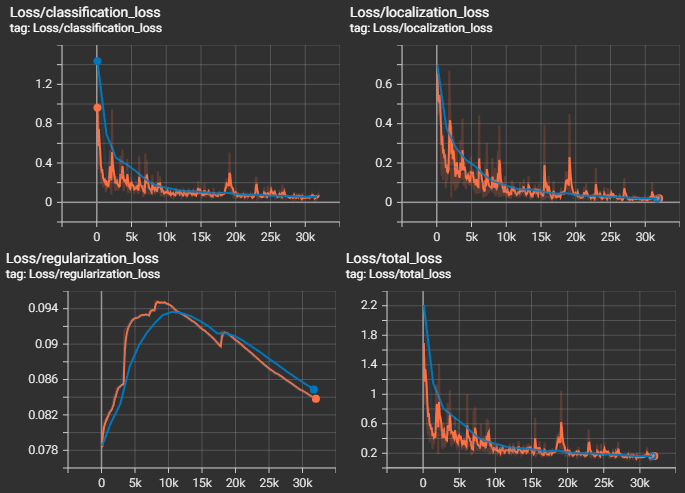
\includegraphics[width=\linewidth]{figure/hand_training.png}}
\caption{Loss curves for the final training of the hand detection model on images from the EPIC KITCHENS dataset.}
\label{hand_training}
\end{figure}

\subsection{Fuzzy Inference System}
In this section we detail the structure of the proposed FIS. Each of the previously discussed input features was created to support an intuitive set of fuzzy rules which were used to produce the final outcome of membership levels in the three action categories of interaction, modification, and relocation.

\subsubsection{Fuzzy Membership Functions}
The input layer of the proposed FIS comprised a set of fuzzy definitions for each of the input features. Tables \ref{inputFeatures} and \ref{outputFeatures} summarize the sets created for the fuzzy input and output features. The two dimensions of the motion vectors were considered as separate fuzzy variables for both frame and object motion. Retaining directional information about the motion was important (as opposed to just the magnitude), and maintaining separate variables per dimension simplified the structure of the system. Each of the other features discussed above was represented by just a single input variable. 

The final number of terms belonging to each input set was initially determined through manual experimentation and knowledge of the feature extraction methods. For example, to compensate for the level of noise expected in the optical flow calculations, a ``low'' membership term was used to represent a lack of significant motion, or motion within an amount of error that a direction could not confidently be determined. 

Triangular membership functions were used for all membership functions within the system in order to keep the definition of the functions as simple as possible, which simplified the encoding of the system for the genetic algorithm discussed later. Trapezoidal functions were tested with no apparent improvement in the results.

\begin{table}
\caption{Input Variables to the Fuzzy Inference System}

\begin{center}
\begin{tabular}{|p{.3\textwidth}|p{.6\textwidth}|}
\hline
\textbf{\textit{Input Linguistic Variable}}&\textbf{\textit{Terms}} \\
\hline
\hline
Frame Motion X (FMX) & \{low (LO), left (L), right (R)\} \\
\hline
Frame Motion Y (FMY) & \{low (LO), down (D), up (U)\} \\
\hline
Object Motion X (OMX) & \{low (LO), left (L), right (R)\} \\ 
\hline
Object Motion Y (OMY) & \{low (LO), down (D), up (U)\} \\ 
\hline
Color Histogram (CH) & \{very low (VLO), low (LO), medium (M), high (HI), very high (VHI)\} \\
\hline
Hand Intersection (HINT) & \{low (LO), high (HI)\} \\
\hline
CenSurE Keypoint (CKP) & \{ low (LO), medium (M), high (HI)\}  \\
\hline
ORB Keypoint (ORB) & \{ low (LO), medium (M), high (HI)\}  \\
\hline
Object Centrality (OC) & \{ low (LO), medium (M), high (HI)\} \\
\hline
\end{tabular}
\end{center}
\label{inputFeatures}
\end{table}


\begin{table}
\caption{Output Variables for the Fuzzy Inference System}

\begin{center}
\begin{tabular}{|p{.3\textwidth}|p{.6\textwidth}|}
\hline
\textbf{\textit{Output Linguistic Variable}}&\textbf{\textit{Terms}} \\
\hline
\hline
Object Interaction (INT) & \{unlikely (UN), somewhat likely (SL), very likely (VL) \} \\
\hline
Object Modification (MOD) & \{unlikely (UN), somewhat likely (SL), very likely (VL) \} \\
\hline
Object Relocation (REL) & \{unlikely (UN), somewhat likely (SL), very likely (VL) \} \\
\hline
\end{tabular}
\end{center}
\label{outputFeatures}
\end{table}


\subsubsection{Fuzzy Rules}
The rules in the fuzzy system control the way in which the inputs are transformed to the outputs. The set of rules used in the system are built intuitively from knowledge of the inputs and how they are expected to change with different activity types. Following is a discussion of the rules in the system grouped by which output action class they relate to.

\paragraph{Interaction}
The level of interaction occurring in a candidate object-action pair was determined by two of the inputs to the system - object centrality, which represents an approximation of the amount of attention being paid to the object by the subject, and hand interaction, which represents an approximation of the amount of hand contact the subject has with the object. The rules affected by these input values are represented in Table \ref{interactRules}.

\begin{table}
\caption{Rules for the Output ``Interaction'' (\textit{HINT}=hand intersection, \textit{OC}=object centrality, \textit{INT}=interaction)}
\begin{center}
\begin{tabular}{cccc}
\hline
\multicolumn{2}{c}{\textbf{\textit{Inputs}}}& &\textbf{\textit{Outputs}} \\
\hline
\hline
\textbf{HINT} & \textbf{OC} & & \textbf{INT}\\
\hline
 LO & & $\longrightarrow$ & UN \\
 & LO & $\longrightarrow$ & UN \\
 & MD & $\longrightarrow$ & SL \\
 HI & & $\longrightarrow$ & VL \\
  & HI & $\longrightarrow$ & VL \\
\hline
\end{tabular}
\label{interactRules}
\end{center}
\end{table}

\paragraph{Modification}
The membership level of the modification output class was determined by the color- and keypoint-based features. The larger the amount of detected change in either feature, the larger the confidence that the action was a modification action. Additionally, the membership of the action in the `interaction' class is considered for the modification class, i.e. if the object was not being interacted with, there should be low confidence that the subject is modifying the object. Note in this case that for the keypoint-based features, the terms `low', `medium', and `high' refer to the level of matching, where low matching would provide stronger support for a change having occurred to the object. The rules affecting the modification output are show in Table \ref{modifyRules}.

\begin{table}
\caption{Rules for the Output ``Modification'' (\textit{INT}=interaction, \textit{CH}=color histogram, \textit{CKP}=CenSurE keypoint similarity, \textit{ORB}=ORB keypoint similarity,  \textit{MOD}=modification)}
\begin{center}
\begin{tabular}{cccccc}
\hline
\multicolumn{4}{c}{\textbf{\textit{Inputs}}}& &\textbf{\textit{Outputs}} \\
\hline
\hline
\textbf{INT} & \textbf{CH} & \textbf{CKP} & \textbf{ORB} & & \textbf{MOD}\\
\hline
LO & & & & $\longrightarrow$ & UN \\
 & VLO & &  & $\longrightarrow$ & UN \\
 & LO & & & $\longrightarrow$ & UN \\
 & & HI & & $\longrightarrow$ & UN \\
 & & & HI & $\longrightarrow$ & UN \\
 & M & & & $\longrightarrow$ & SL \\
 & & M & & $\longrightarrow$ & SL \\
 & & & M & $\longrightarrow$ & SL \\
 & HI & & &  $\longrightarrow$ & VL \\
 & VHI & & & $\longrightarrow$ & VL \\
 & & LO & & $\longrightarrow$ & VL \\
 & & & LO & $\longrightarrow$ & VL \\
\hline
\end{tabular}
\label{modifyRules}
\end{center}
\end{table}

\paragraph{Relocation}
The motion features naturally formed the basis for the output membership level in the relocation class. Similarly to the modification rules, the level of interaction informs the level of relocation, since it is assumed that a relocation cannot occur without an interaction. The rules affecting the relocation output are show in Table \ref{relocateRules}. For rules with multiple inputs on the same line are created using the conjunctive operator AND.

The rules effectively form a differencing operation between the object and global frame motion. While the difference could have been computed prior to entering the fuzzy system, cutting the number of rules required, the differencing was performed within the fuzzy system to retain as much of the input information as possible in the event that the information became pertinent to another rule.

\begin{table}
\caption{Rules for the Output ``Relocation'' (\textit{OMX}=object motion in x direction, \textit{OMY}=object motion in y direction, \textit{FMX}=frame motion in x direction, \textit{FMY}=frame motion in y direction, \textit{INT}=interaction, \textit{REL}=relocation)}
\begin{center}
\begin{tabular}{ccccccc}
\hline
\multicolumn{5}{c}{\textbf{\textit{Inputs}}} & & \textbf{\textit{Outputs}} \\
\hline
\hline
\textbf{OMX} & \textbf{OMY} & \textbf{FMX} & \textbf{FMY} & \textbf{INT} & & \textbf{REL}\\
\hline
 & & & & LO & $\longrightarrow$ & UN \\
L & & L & & & $\longrightarrow$ & UN \\
R & & R & & & $\longrightarrow$ &  UN \\
& U & & U & &$\longrightarrow$ &  UN \\
& D & & D & &$\longrightarrow$ &  UN \\
LO & & LO & & & $\longrightarrow$ & UN \\
 & LO & & LO & & $\longrightarrow$ & UN \\

 L & & $\neg$ L & & & $\longrightarrow$ & VL \\
 R & & $\neg$ R & & & $\longrightarrow$ & VL \\
 & U & & $\neg$ U & & $\longrightarrow$ & VL \\
 & D & & $\neg$ D & & $\longrightarrow$ & VL \\
 LO & & $\neg$LO & & & $\longrightarrow$ & VL \\
 $\neg$LO & & LO & & & $\longrightarrow$ & VL \\
 & LO & & $\neg$LO & & $\longrightarrow$ & VL \\
 & $\neg$LO & & LO & & $\longrightarrow$ & VL \\
\hline
\end{tabular}
\label{relocateRules}
\end{center}
\end{table}

\subsubsection{Fine Tuning with Genetic Algorithm}
While the inputs, outputs, membership functions, and rules described thus far were built on intuition and experimentation within the problem domain of activity classification, there still remained possibility for optimizing the performance of the system. The optimization was performed by using a genetic algorithm to evolve the membership functions for each variable in the system. 

While the FIS derives power from interpretability and explainability of the results, tuning the membership functions with a GA does not remove these benefits. It is difficult to intuitively determine, for example, where the lower or upper bounds of a membership function should reside for a `low' movement term. Clearly the relation of `low' to `high' is intuitive, but the number of pixels of motion per frame that should represent `low' amounts of motion is unclear. The GA provides a method of extracting sensible values for each membership function while optimizing the performance of the system.

\paragraph{Genetic Representation}
In order to evolve the FIS using a GA, a genetic/chromosomal representation of the functions defined within the system was required. Since the triangular membership function for each term was defined by a set of three values representing the lower, middle, and upper extents of the triangle, a real-valued triplet encoding was used to encode each function. The entire gene, then, was represented as a collection (dictionary) of real-valued triplets. An excerpt of one such genetic representation is provided in Listing \ref{genetic_rep}. This is represented in short form as a nested list of values: $\{[-3.915, -3.00, 2.424], [-2.353, -0.132, 2.024], [-2.799, 3.477, 3.794], ...\}$

\begin{lstlisting}[language=Python, basicstyle=\small, columns=flexible, frame=single, label=genetic_rep, caption=Example JSON for Genetic Representation]
{
  ``frame_movement_x'': {
    ``left'': [-3.915, -3.000, 2.424], 
    ``low'': [-2.353, -0.132, 2.024], 
    ``right'': [-2.799, 3.477, 3.794]
  }, 
  ``obj_movement_x'': {
    ``left'': [-3.820, -3.729, 3.868], 
    ``low'': [-3.655, 0.786, 2.917], 
    ``right'': [1.096, 3.00, 4.258]
  },
...
}
\end{lstlisting}

For the process of evolving a high-accuracy solution, the population was initialized with 20 randomized individuals. Each individual was tested against a set of 3,560 actions from the EPIC KITCHENS dataset to evaluate fitness. The actions were sampled from 7 different videos. In an attempt to retain negative prediction value, annotations of objects with no action were also included in this training set since many objects in the scene may be part of no action.

Roulette wheel selection was used to select parents for new generations, meaning that each parent had a chance of selection proportional to their fitness relative to the fitness of the other individuals. Single-point crossover was used in the mating process, and mutation occurred with a probability of $p=0.20$. When selected for mutation, a value in the system was allowed to randomly move within $\alpha=1.2$ times the distance to it's neighbors. Since $\alpha > 1$, it was possible for a term to surpass it's neighbor. This was allowed in order to not constrain the evolutionary process. As an implementation detail, care had to be taken to keep the system well-formed, e.g. that the lower bound on a triangular function did not become greater than an upper bound. Following all mutations, the values in each triplet were re-sorted to ensure that the lower, middle, and upper values were appropriately ordered. In this way, a mutated lower value was able to become the middle value of a triangle if it happened to mutate past the original middle value, and so on.

Several fitness functions were experimented with during the training process. As is the case with any classification problem, the accuracy of the system must be weighed against the impact of different types of errors. Training for high accuracy often led to a bias in positive or negative results for a particular category, but the F1 score provided an appropriate balance between accuracy, precision, and recall and was ultimately used as the fitness metric during training.

\subsection{Results}
This section provides details on the results of the methods used to classify activities using the FIS, including the custom built hand detector, the tuning of the FIS with genetic algorithms, and finally the overall results of classifying activities with the FIS.

\subsubsection{Hand Detection}

\begin{figure}[t]
\begin{subfigure}{.5\textwidth}
\centerline{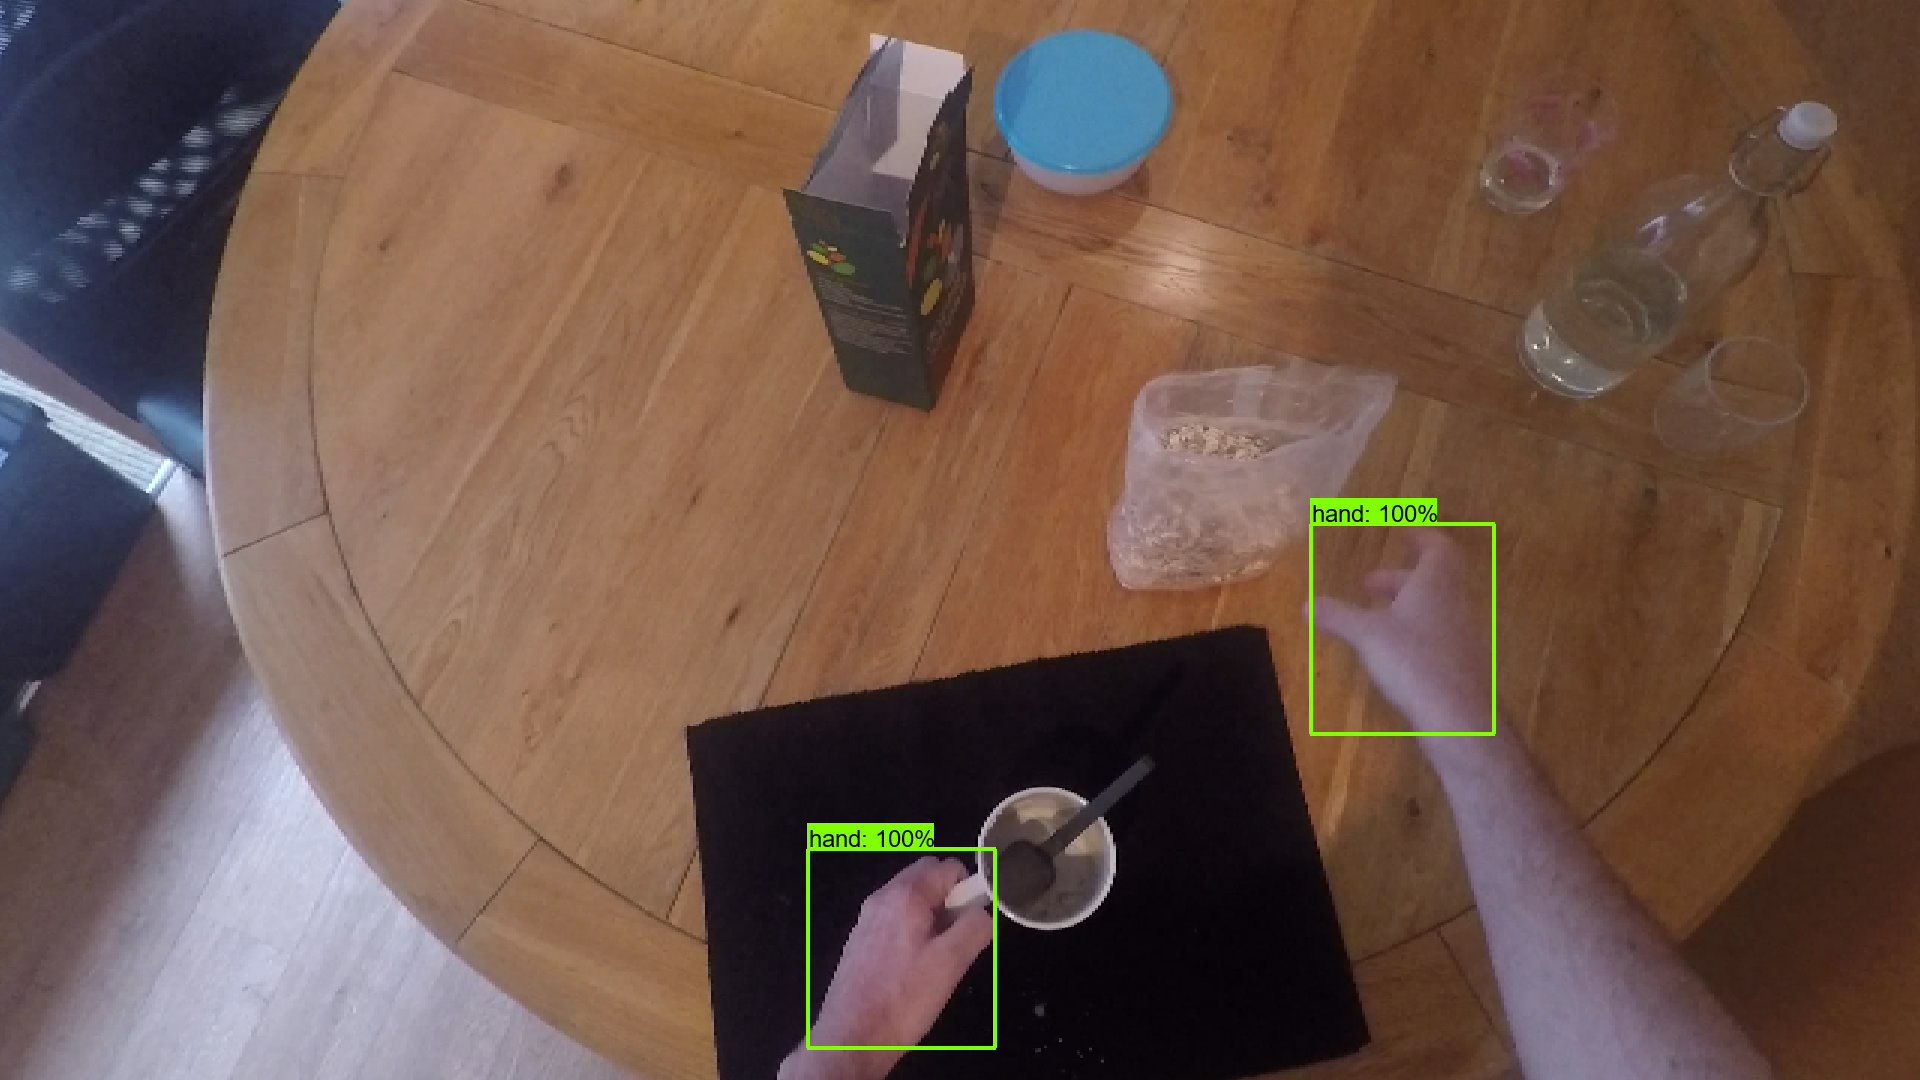
\includegraphics[width=.95\linewidth]{figure/handEval1.png}}
\label{handsA}
\end{subfigure}
\begin{subfigure}{.5\textwidth}
\centerline{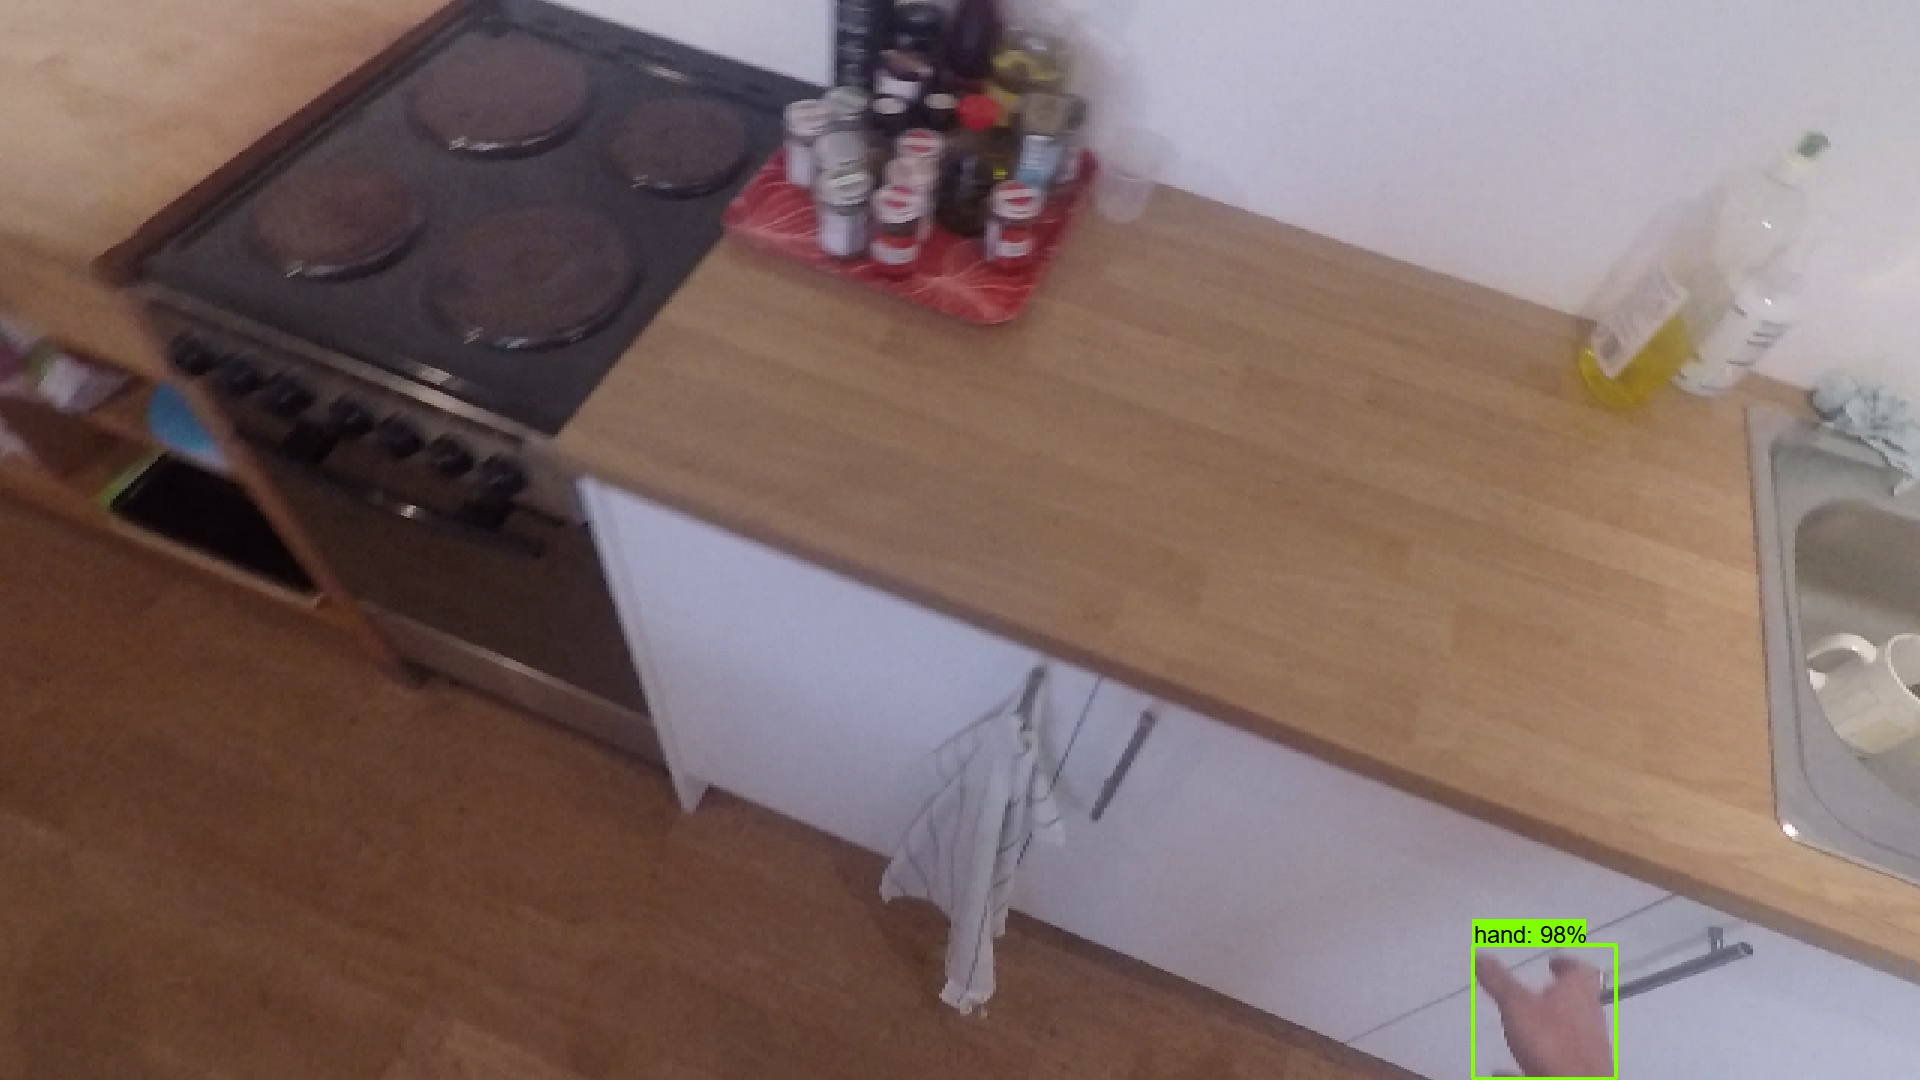
\includegraphics[width=.95\linewidth]{figure/handEval2.png}}
\label{handsB}
\end{subfigure}
\\ 
\begin{subfigure}{.5\textwidth}
\centerline{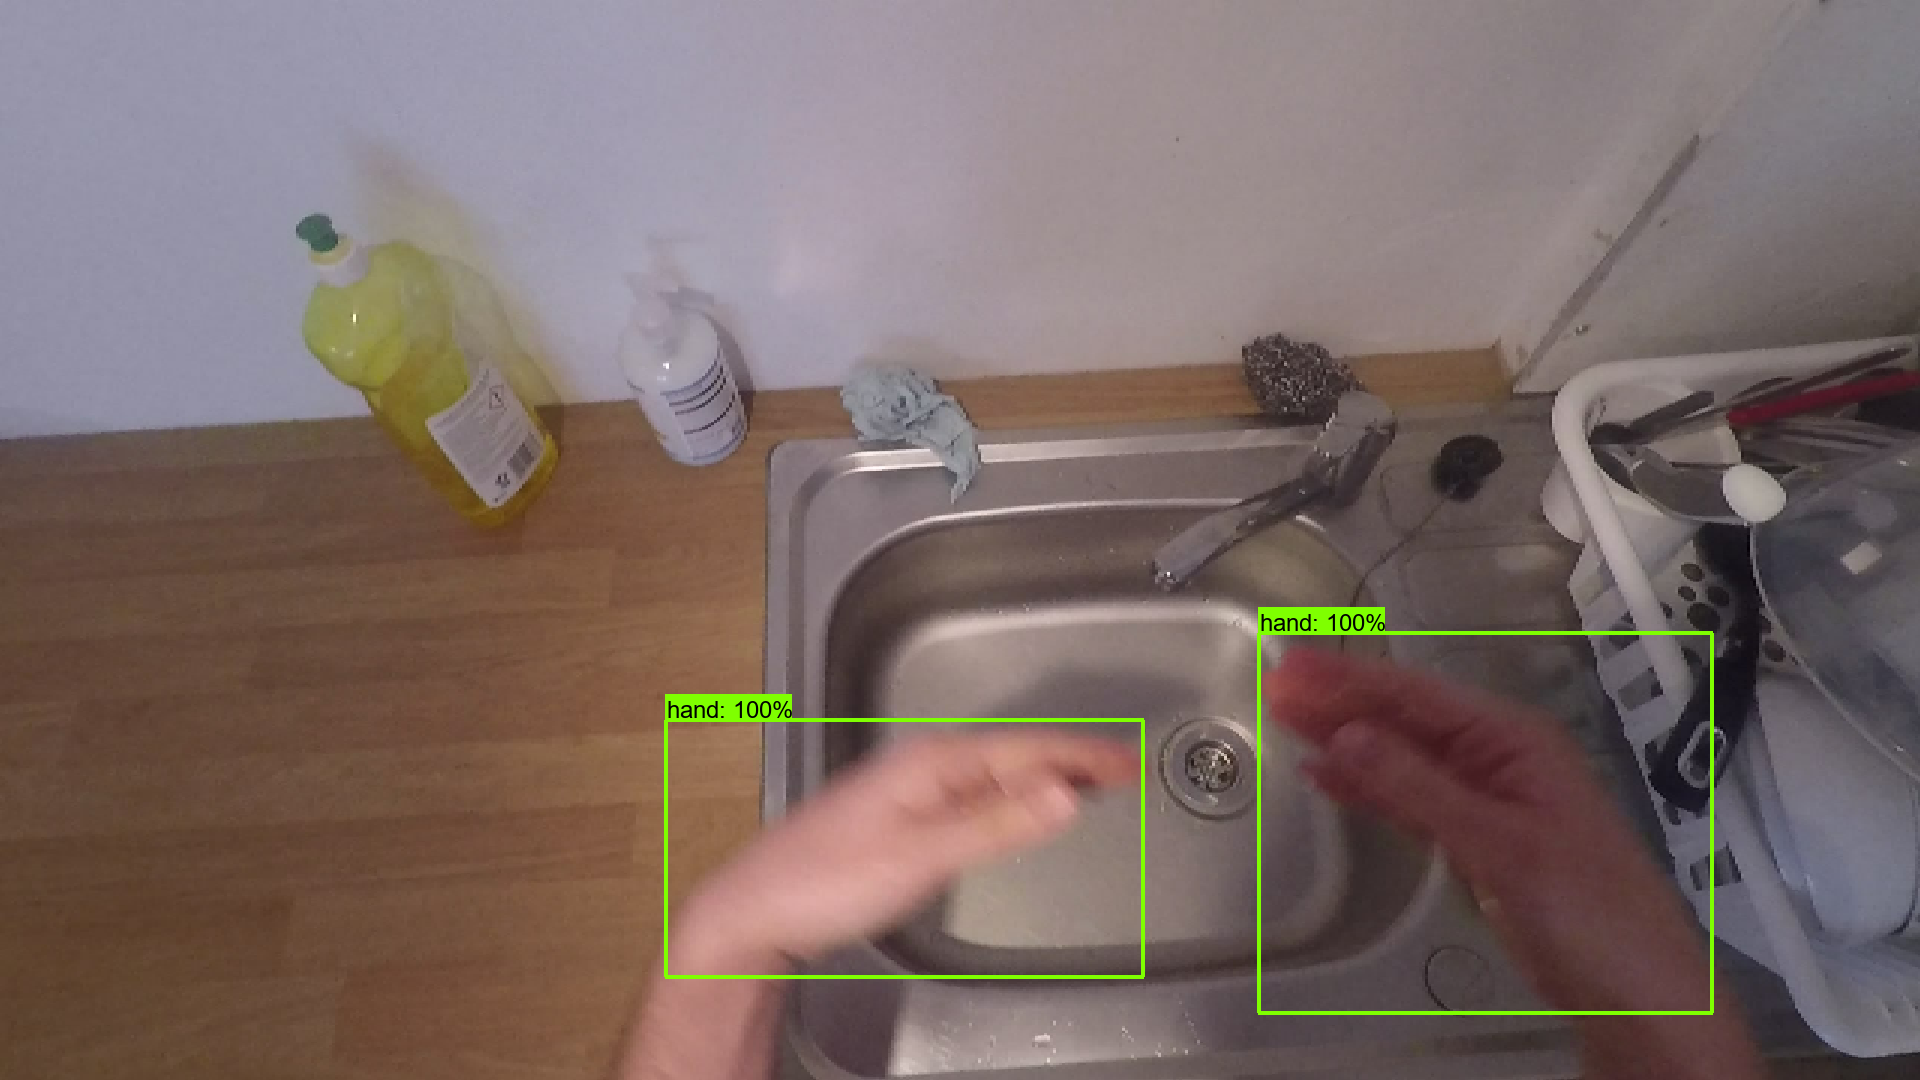
\includegraphics[width=.95\linewidth]{figure/handEval3.png}}
\label{handsC}
\end{subfigure}
\begin{subfigure}{.5\textwidth}
\centerline{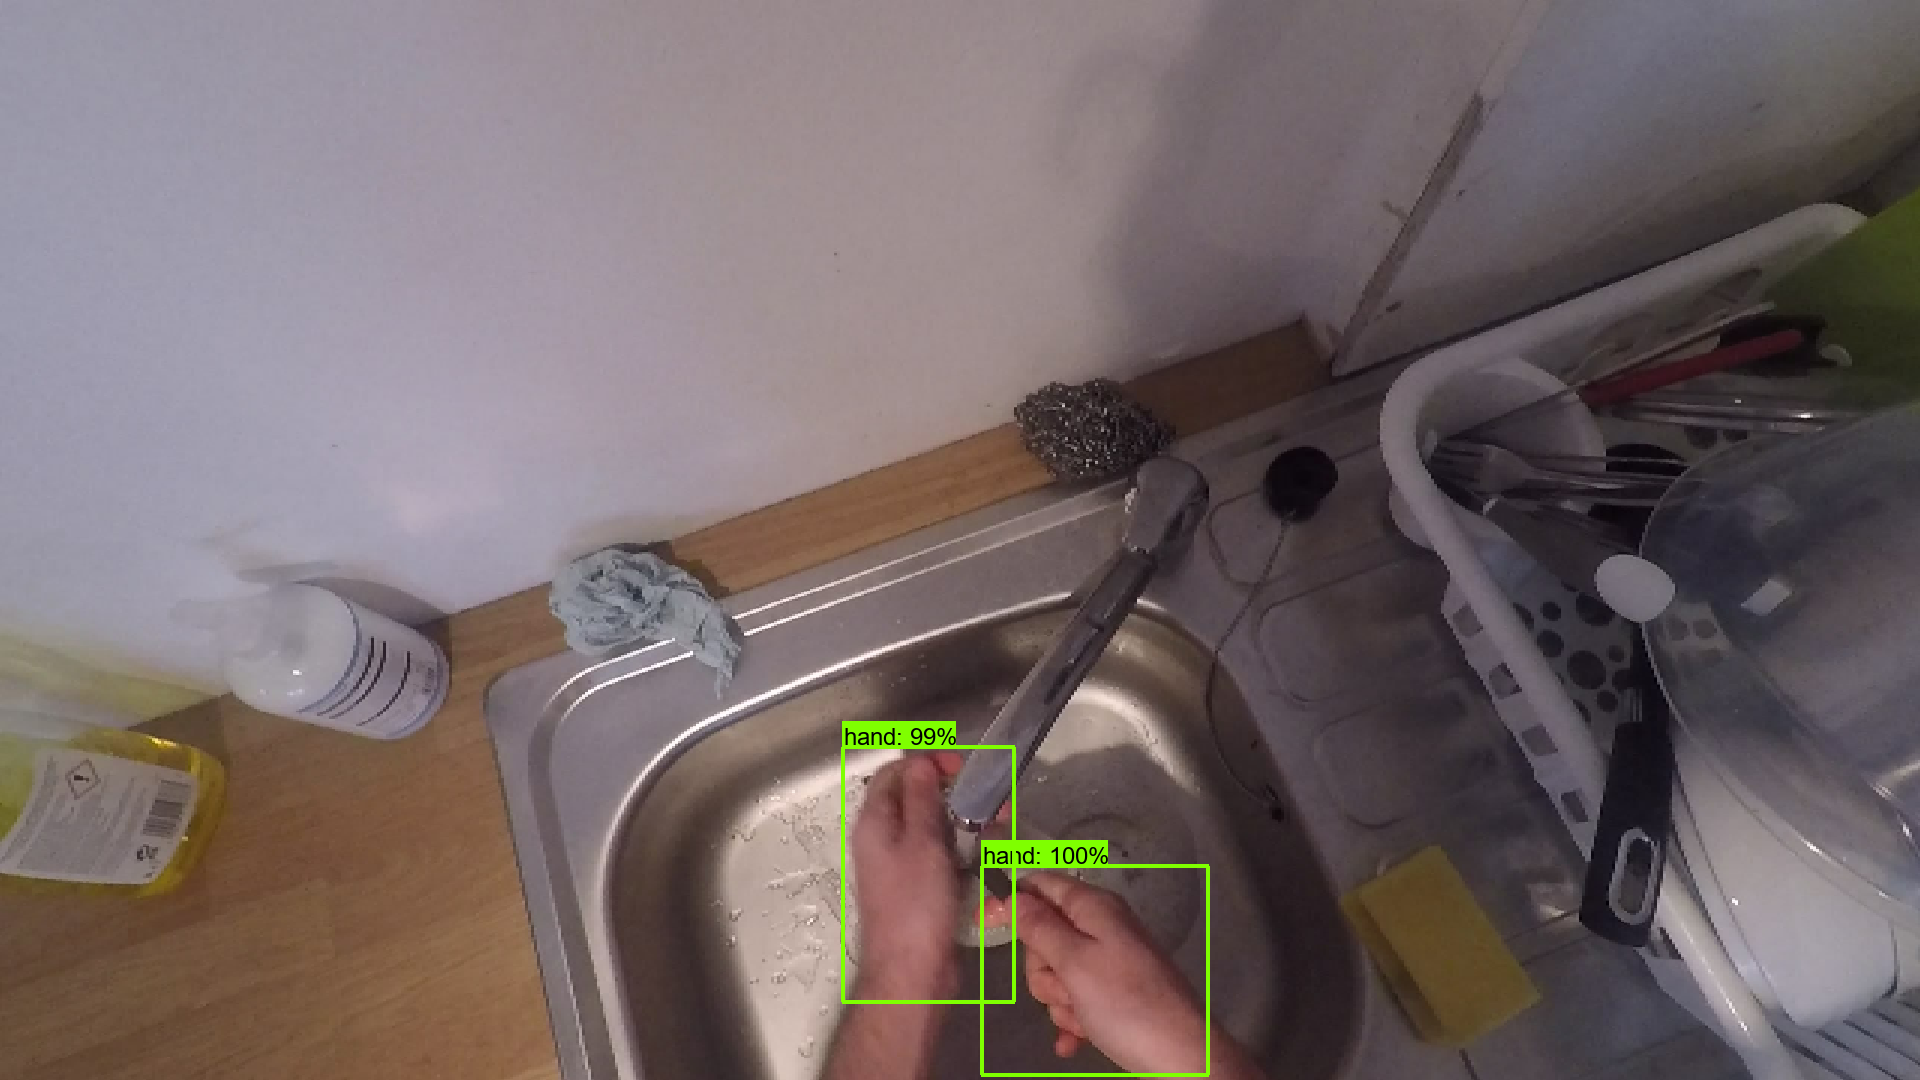
\includegraphics[width=.95\linewidth]{figure/handEval4.png}}
\label{handsD}
\end{subfigure}
\caption{Example first-person video frames of the hand detection model. Hands were detected in these images with a confidence ranging between 0.96 to 1.0, highlighting the robustness of the model to different orientations and poses of hands in the view.}
\label{sampleFrame}
\end{figure}


\subsubsection{Genetic Algorithm Tuning}


\subsubsection{Fuzzy Action Classification}

We evaluated our work against a set of eight videos from the Epic Kitchens dataset \cite{Damen2018ScalingDataset}. This dataset contains unscripted first-person videos of subjects performing daily activities such as cooking, washing dishes, and cleaning in their kitchens. Annotations of objects and actions occurring on the objects are provided every 30 frames. The action annotations provided with the dataset comprise over 100 different verbs. For the purpose of evaluating results against the annotated truth, we binned each annotated truth action into one of three action categories reflecting the fuzzy output variables - interaction, modification, and relocation. While our expectation is that actions will have some membership in more than one output category, for current evaluation purposes we chose the annotated truth for each verb based on the category from which the strongest membership is expected. 

The selected videos contain 4310 action annotations, where each action annotation is defined as a tuple of one of 43 unique verbs and one of 56 unique nouns. Of these actions, 1711 were annotated as `interact', 1225 were annotated as `modify', and 977 were annotated as `relocate'. Table \ref{results} summarizes the results for each class of activity.

From Table \ref{results}, we observe that the fuzzy system produces the highest precision (0.523), recall (0.771), and f1 (0.623) metrics for actions in the `interact' class. However, the specificity for the `interact' class is the lowest (0.537), suggesting that the fuzzy system is identifying a sizeable proportion of false negatives along with the true positives in this class. This indicates that our current system is very sensitive to the true positives with a higher recall but performing poorer due to a higher rate of false positives.

On the flip side, our fuzzy system produced the highest specificity metric for the `relocate' class with a specificity of 0.705. The system is identifying a much lower rate of false positives for this class, but this comes at the expense of identifying true positives; this class also has the lowest precision (0.148), recall (0.175), and f1 (0.160) scores. This indicates that there is a need for further parameter tuning to improve model performance.

Our use of the annotations provided with the dataset also introduces some amount of undesirable noise into the input features. For example, the annotated bounding boxes provided with the dataset are imprecise and only updated every 30 frames; Figure \ref{sampleFrame} illustrates two issues with the bounding box annotations - first, the loose fit of the rectangular bounding box to the objects (Figure \ref{sampleA}), which introduces noise in the object motion input features, and second, the low frequency of updates to the bounding box which produces a poor result when the object moves out of the are before the bounding box is updated (Figure \ref{sampleB}).

The current rules implemented in our system are based on a relatively small amount of information from the video, which limits the ability to properly classify activities in more complex scenes, such as when the image is poorly lit, blurry, or otherwise obscured. A system with more features will be better equipped to tolerate this noise.

While the accuracy of our fuzzy system does not exceed the accuracy reported in related work using supervised classification techniques such as deep learning, the system is competitive with their results and shows potential for use after further refinement \cite{Pirsiavash2012, Koppula2016, Lu2019}. The set of features being supplied to our system is small, and those features are simple yet explainable. A set of more robust features is likely to improve the performance of the system. For example, the hand segmentation feature is computed by a simple color segmentation algorithm. Replacing this with a more robust detection of the hand position will give a more reliable result. Similarly, the use of more complex motion features, per-frame annotations, and non-rectangular bounding boxes are all future work that would improve the classification results.

\begin{table}
\caption{Results of activity classification on first-person video}
\begin{center}
\begin{tabular}{cccccc}
\hline \\
\textbf{\textit{Activity Class}} & \textbf{\textit{precision}} & \textbf{\textit{recall}} & \textbf{\textit{f1}} & \textbf{\textit{specificity}} \\
\hline
interact & 0.523 & 0.771 & 0.623 & 0.537 \\
modify & 0.265 & 0.325 & 0.292 & 0.642 \\
relocate & 0.148 & 0.175 & 0.160 & 0.705 \\
\hline
\end{tabular}
\label{results}
\end{center}
\end{table}

\begin{figure}[t]
\begin{subfigure}{.5\textwidth}
\centerline{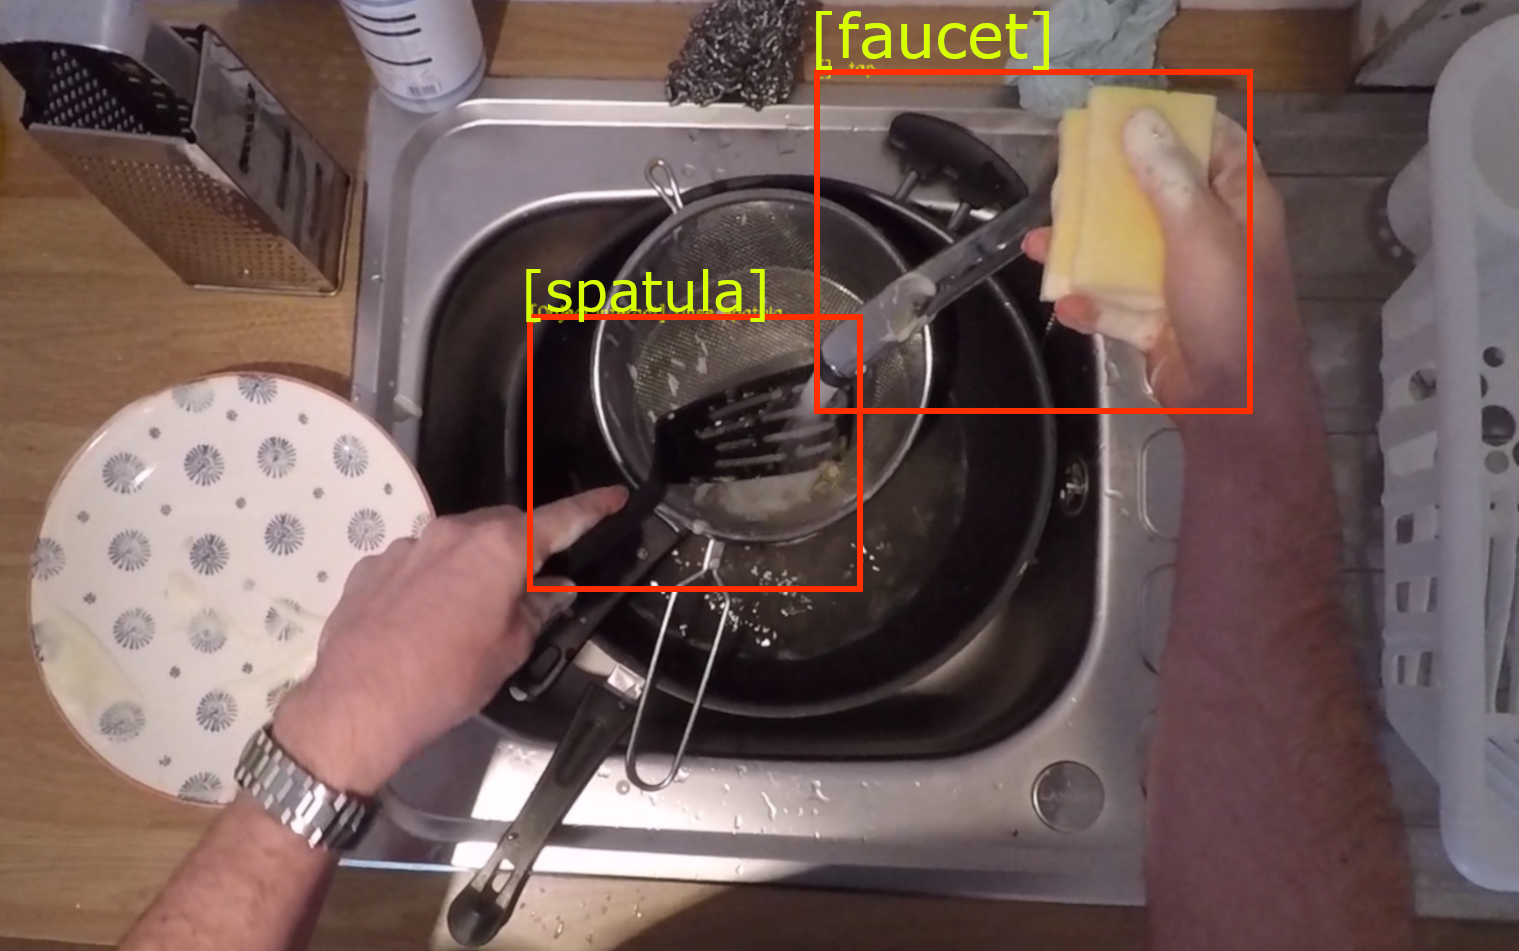
\includegraphics[width=.8\linewidth]{figure/frame_4085_cropped.png}}
\caption{Video frame with loose rectangular bounding boxes around a spatula and faucet}
\label{sampleA}
\end{subfigure}
\begin{subfigure}{.5\textwidth}
\centerline{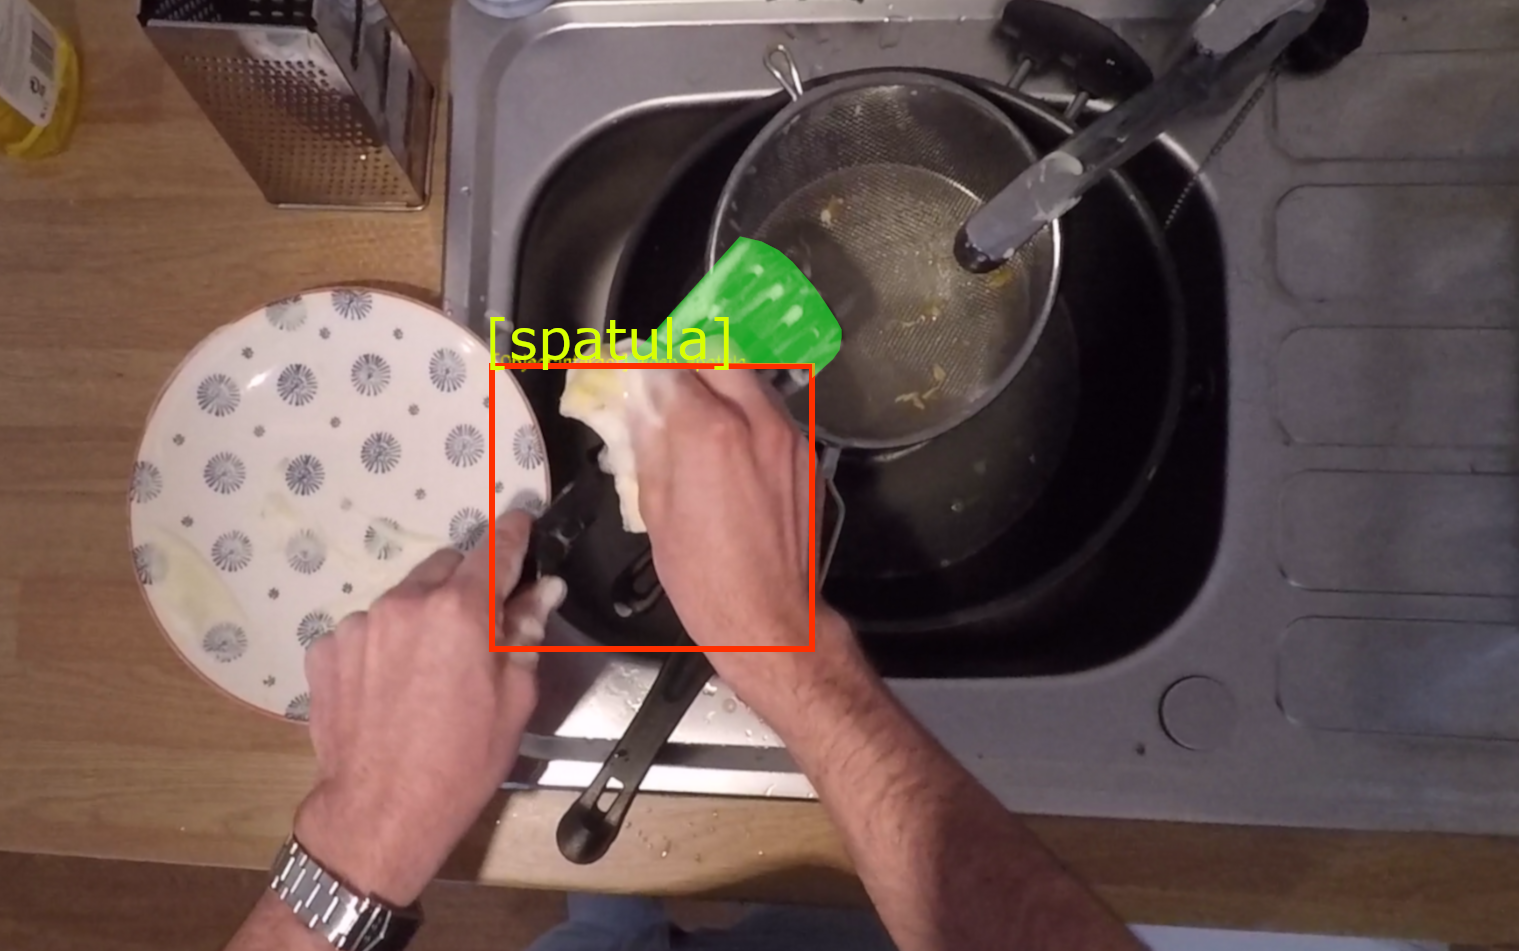
\includegraphics[width=.8\linewidth]{figure/frame_4527_cropped.png}}
\caption{Video frame with object exceeding the rectangular bounding box (the portion of the spatula outside of the bounding box is highlighted in green)}
\label{sampleB}
\end{subfigure}
\caption{Example first-person video frame of subject washing spatula with overlaid bounding boxes, action, and object labels}
\label{sampleFrame}
\end{figure}

During the analysis of our results, we also observed subjectivity in the human-generated action annotations provided with the dataset. The annotation of actions on a per-frame basis is very difficult since there is rarely a definitive start and end to an activity at such close temporal resolution. We observed inconsistencies in the application of action labels stemming from the imprecision of natural language. For example, opening a faucet, opening a refrigerator, and opening a bottle are very different types of actions and motions from the subject. While the verb for each of these actions is the same, they are clearly not the same action. The variance seen between these results via the membership in our fuzzy outputs captures the difference much more precisely than the verb label. Thus, we have identified a possible application of fuzzy methods in the refining of annotated truth.

\subsection{Conclusions}
In this experiment, we took a novel approach to egocentric action classification through the use of a fuzzy inference system, highlighting the potential for the use of the system for in-home monitoring. While the features that were input to the fuzzy system were relatively simple, the system was able to provide fuzzy membership of actions in three unique action categories - object interaction, relocation, and modification - which describe the nature of the interaction. Our evaluation of the system against a set of 4310 unscripted actions revealed the possibility of enhanced action descriptions through fuzzy memberships. This derived understanding can be used for in-home activity analysis in geriatric case, assisted living, or hospital settings. Our evaluation also revealed potential for enhancing the action annotation process. The fuzzy output variables bring the potential to provide a richer description of both atomic and complex activities through varying membership levels in several classes.

Future work with this fuzzy system will involve further parameter tuning using genetic algorithms and enhancing the complexity and number of input features to allow for more complex rules, which will in turn provide a more reliable classification result.




%================================================
\chapter{Proposed Future Work}
%================================================
The work described thus far provides introduction and motivation for our problem of describing activities in first-person video, a review of related works in the field including sensor hardware, types of activities, and computational intelligence methods used, an overview of the proposed methods, and the description and results of previous experiments motivated by our research questions. 

While we can see conclusions from completed experiments relating to the first two research questions posed in the Introduction, Research Question 3 (\emph{Can the activity identification system a) accurately describe activities and b) handle uncertainty in the results better than current state-of-the-art methods?}) necessitates further work to improve the accuracy of the fuzzy system described in section 4.2 and to address the question of whether the system handles uncertainty in activity classification results (i.e. whether the system provides enhanced explainability of the results even when the classification is unknown or incorrect).

\section{Timeline}
Remaining activities which are expected to provide a satisfactory response to the outstanding research questions are outlined in Figure \ref{timeline}.

%\begin{landscape}

\begin{figure}
\noindent\resizebox*{\linewidth}{!}{ % Rescale the chart to linewidth
\begin{ganttchart}[vgrid, hgrid, x unit = 1cm]{1}{13}
\gantttitle{2020}{9}
\gantttitle{2021}{4} \\
\gantttitlelist{4,...,12}{1}
\gantttitlelist{1,...,4}{1} \\
\ganttbar{Proposal Defense}{1}{1}\\
\ganttbar{Optimization of Fuzzy Rules using GA}{1}{2} \\
\ganttgroup{Enhancements to Input Features}{2}{7} \\
\ganttbar{Hand recognition with NN}{2}{3} \\
\ganttbar{Advanced Optical Flow Features}{4}{5} \\
\ganttbar{Object Change Features}{6}{7} \\
\ganttbar{Further Rule Discovery and Optimization}{8}{8} \\
\ganttbar{Evaluation of System}{9}{9}\\
\ganttbar{Update Dissertation Document}{10}{11} \\
\ganttbar{Review and Edit Document}{12}{12} \\
\ganttbar{Final Defense}{13}{13} \\
\end{ganttchart}
}
\caption{Proposed project timeline}
\label{timeline}
\end{figure}

A brief description of the events follows:
\begin{itemize}
    \item Optimization of Fuzzy Rules using GA: Refinement and tuning of the existing set of fuzzy rules using genetic algorithms to evolve the membership functions \cite{Tan1999OptimizationRating}. This method optimizes the effectiveness of the existing rules.
    \item Enhancments to Input Features
    \begin{itemize}
        \item Hand recognition with NN: Detecting hands in the video is a strong driver of the classification result. Color segmentation methods were originally chosen for simplicity but are not sufficient across lighting conditions and skin tones. Work has been started on using a neural network to recognize hands with some initial improvement but requires additional tuning to be more effective.
        \item Advanced Optical Flow Features: More complex optical flow-based features have been used in related work \cite{Ryoo2015, Abebe2016}, and these may provide a richer source of data from the observed scene.
        \item Object change features: The use of the color histogram to detect change in an object's appearance may only be reliable for sudden or sharp changes in appearance. Additional object shape descriptors and methods of comparing objects' appearances over time will likely improve the performance of the system.
    \end{itemize}
    \item Further rule discovery and optimization: Following the implementation of new features, a second round of rule optimization and tuning is expected since the new features require new rules.
\end{itemize}

%\end{landscape}

%%=============================
%\chapter{In The Beginning}
%%=============================
%The date of this document generation (current version of this document) is the date of the thesis on page two (\today).{}
%sdafsd sadfsdaf asdfadf. OK, I have nothing to say here, but you should in your thesis/dissertation. Introduce your chapter in a page or so.
%
%On a side note, style files should be located in the texmf tree automatically when a package is installed.  The sty-files used for this template are located in the folder \lq\lq{}sty\_files\_if\_needed\rq\rq{}.  If you do not have the packages already installed, you can also simply move or copy them into the same directory as this file.
%
%%=============================
%\section[Citations/References (short form of section name)]{Citations, using them, referring to them, formatting them, and loving using them because if you don't use them when appropriate it's called \emph{plagiarism}, and references}
%%=============================
%That was a ridiculously long section name to illustrate how to get a shorter version in your table of contents.
%
%See Section~\ref{sec:equations}. I'm not the only one who says this is awesome stuff\cite{Mortara2004}!
%This citation is in the ASME format for which I've included a \verb'bst'
%file. See \textsc{asmems4} in the source document (way near the end). Some  other options are:
%\begin{itemize}
%\item natbib:  put \verb'\usepackage{natbib}' in the header (before \verb'\begin{document}'), and \verb'\bibliographystyle{plainnat}' (just before \verb'\bibliography').  See the natbib documentation for details.
%\item AIAA:\@put \verb'\usepackage{overcite}' in the header (before \verb'\begin{document}'), and \verb'\bibliographystyle{aiaa}' (just before \verb'\bibliography'). Use \verb'\citen{sdfsdf}' for in-line citations. Read the overcite package documentation for more.
%\end{itemize}
%
%A variety of other formats are available on \href{http://www.ctan.org}{CTAN} or though an internet search. You may also just pick one using ``natbib''.\footnote{Don't those quotes look bad before ``natbib''? Well, use two left quotes in \LaTeX\ to get it to look right.}  The formatting of your references is controlled by the \verb'bibliographystyle' command near the end of the document. Use the bibliography style appropriate to your field. On exists, out there. I'm sure. If not (ok, it happened to me 10 years ago), you can use the \verb'makebst' script to make your own. Answer a bunch of questions and it makes a style file for you. If you are using a numerical citation system, you may want to use \verb'\usepackage{cite}'. It creates a condensed numerical list of citations, but can cause conflicts with the \verb'hyperref' package (you may need to decide\ldots sorry, this is a bug that drives me nuts too.)
%
%%=============================
%\subsection{About the Bibliography}
%%=============================
%There are two lines in this section in your \LaTeX\ file. The first is a bibligraphystyle command (see the \textsf{tex} file. Don't move it elsewhere. It won't work out well for you.
%
%You need to choose a style file that formats references the way you want them formatted.  You should chose a style for your major.  Look for bst styles on ctan, or use makebst.sty. This formats the bibliography.
%The last line is the bibliography command. It just tells \LaTeX\  the name of your \textsf{.bib} file. This is a database of your references.
%
%Also, use the \verb'\phantomsection' command to correctly anchor the hyperlink for the bibliography.  Without this, any hyperlinks in the document, and the link from the bookmarks will take you to the incorrect page.
%
%You can have as many sources listed in the *.bib file, but if you do not cite them in your document, they will not show up in your Bibliography.  And if you do, they automatically are sorted\ldots pretty nice!
%
%%=============================
%\subsection{Equations}\label{sec:equations}
%%=============================
%\begin{equation}\label{eq:alphaoverbeta} %You can name the label anything you want, just not the same as something else
%x=\frac{\alpha}{\beta}
%\end{equation}
%Really bad idea: don't start a section with an equation. Don't start a sentence with a variable either. Start with a word. In the body of the text, use the \$ around the variable.  For example, the variable $x$ is the distance. How hard was that?
%
%Sometimes you don't want an equation  number, so use \verb'{equation*}' instead.
%\begin{equation*}
%x=\frac{-b\pm\sqrt{b^2-4ac}}{2a}
%\end{equation*}
%
%If you need to align a set of equations up use the \verb'align' command instead with the use of the \& to set the anchor
%\begin{align}
%x&=\frac{-b\pm\sqrt{b^2-4ac}}{2a}\\
%x&=\frac{\alpha}{\beta}
%\end{align}
%The same applies for the \verb'align' command\ldots if you don\rq{}t want equation numbers,  just use an *.  More can be found at the references listed in Section~\ref{sec:refs}.  You can easily make matrices such as the viscous damping matrix, $C_d$, which is shown in Equation~\eqref{eq:damping_mat}.  Use the \verb'\eqref{eq:\ldots}' command to reference equations properly.
%%
%\begin{equation}
%\label{eq:damping_mat}
%C_{da} =[U_n^Tnn]^{-1}
%\left[ \begin{array}{ccc}
%a&b&c\\
%	\ddots & 				& \\
%	     	& 2 \zeta_i \omega_i 		& \\
%		&				& \ddots \\
%\end{array} \right]^{{-1}} [U_n]^{-1}
%\end{equation}
%
%We don't number equations in \LaTeX. \LaTeX\ does it for us. Label them with names (see the raw \LaTeX\ file).   Just don't put a space in the middle of a variable name.
%
%Now if I have an equation that I want to be between paragraphs, unlike equation (\ref{eq:alphaoverbeta}), I put a blank line after the equation.
%\begin{equation}
%  \label{eq:anothersillyequation}
%  x\neq y
%\end{equation}
%
%See  indent? But if I'm continuing the paragraph, don't put that blank line in
%\begin{equation}
%  \label{eq:anothersillyequation2}
%  x\neq y
%\end{equation}
%and there won\rq{}t be an indent.
%
%If you want a new page and you have a figure you want to stay with the section, you need to use the \verb'\clearpage' command instead of the \verb'\newpage' command.
%
%%=============================
%\section{Figures}
%%=============================
%This is not the same as Section~\ref{sec:equations} on equations. However, if I move that section, I'll still be referring to the right section.
%Better explained by Figure\footnote{a- Don't use footnotes.\ b- Capitalize the word ``Figure''}~\ref{fig:example}.  You can keep all of your figures in a sub-directory such as \lq\lq{}pix\rq\rq{}, which is used in this template.
%\begin{figure}[htbp] %  figure placement: here, top, bottom, or page
%   \centering
%   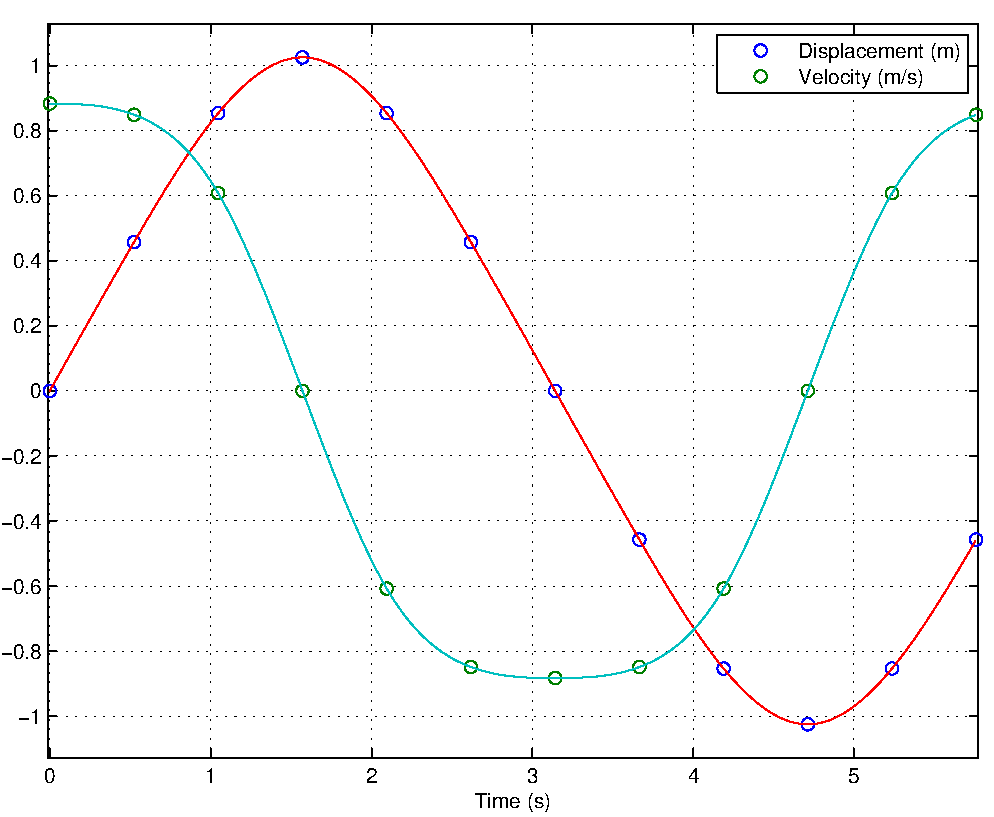
\includegraphics[width=.5\textwidth]{WSUThesisTemplate/pix/example.pdf} %
%   \caption{Example caption.}
%\label{fig:example}
%\end{figure}
%
%The width of the figure can be set based on percentage of text width as set in Figure~\ref{fig:example} or based on inches as used in Figure~\ref{fig:example2}.  Also notice the \verb'\label' is after the \verb'\caption'.  This must be true, or the hyperlinks and figure numbers will not be correct.
%
%%----------------------------------------------------------
%\begin{figure}[!t] %forced to top of page so no text will be stranded above
%   \centering
%   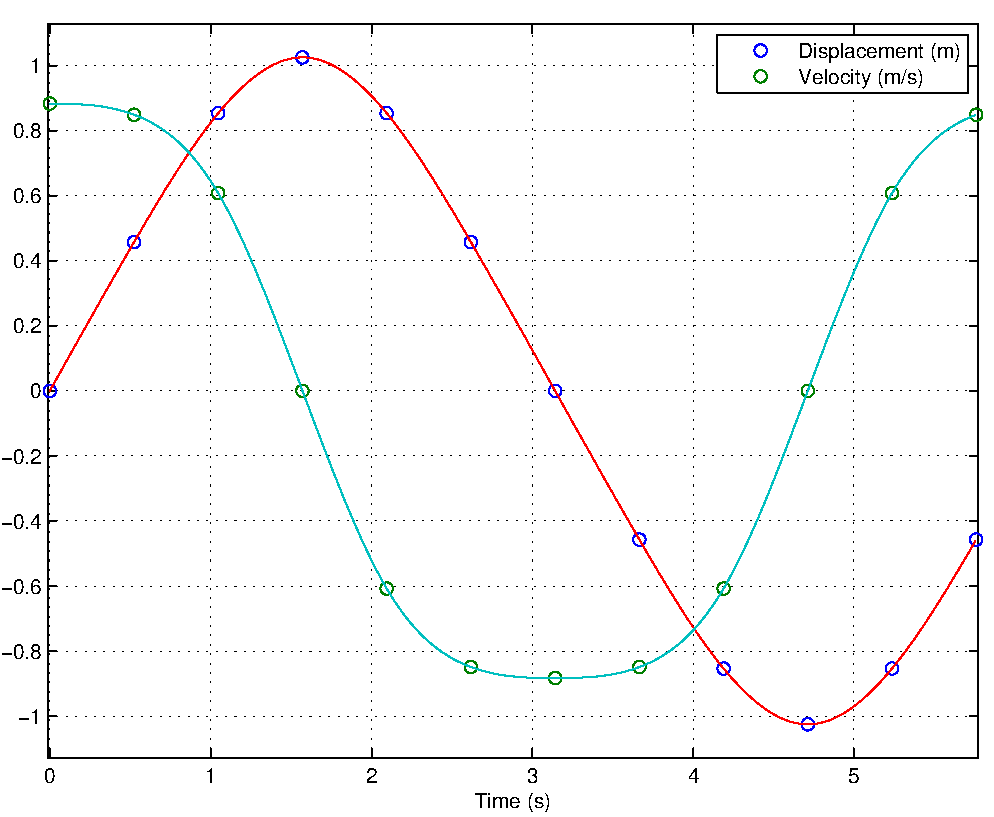
\includegraphics[width=3in]{WSUThesisTemplate/pix/example.pdf} %
%   \caption[Short Figure Caption]{Example caption that is way too long for the list of figures, is a run on sentence, has no purpose being this long, except to show you how to avoid such a crazy long entry in your list of figures.}
%\label{fig:example2}
%\end{figure}
%%----------------------------------------------------------
%
%Don't ask me why the label command has to come late in a figure. It does.  Remember, color won't print well in black and white. Use dashes and dash-dots, etc, for hard copies. I'll document a trick for this later. Basically, make two graphics directories, one for color, one for black and white. Then, use the \textsf{graphicspath} command to choose the one you want. You can Google this for now.
%
%%=============================
%\section{Sub-figures}
%%=============================
%You can also make sub-figures and reference each of them individually.  You can reference the entire Figure~\ref{fig:1x2_subfigs}, or just Figure~\ref{fig:example_a} or Figure~\ref{fig:example_b}.
%%-----------------------------------------------------------------
%\begin{figure}[!ht]
%  \centering
%  \subfigure[First sub-figure]{
%\label{fig:example_a}
%   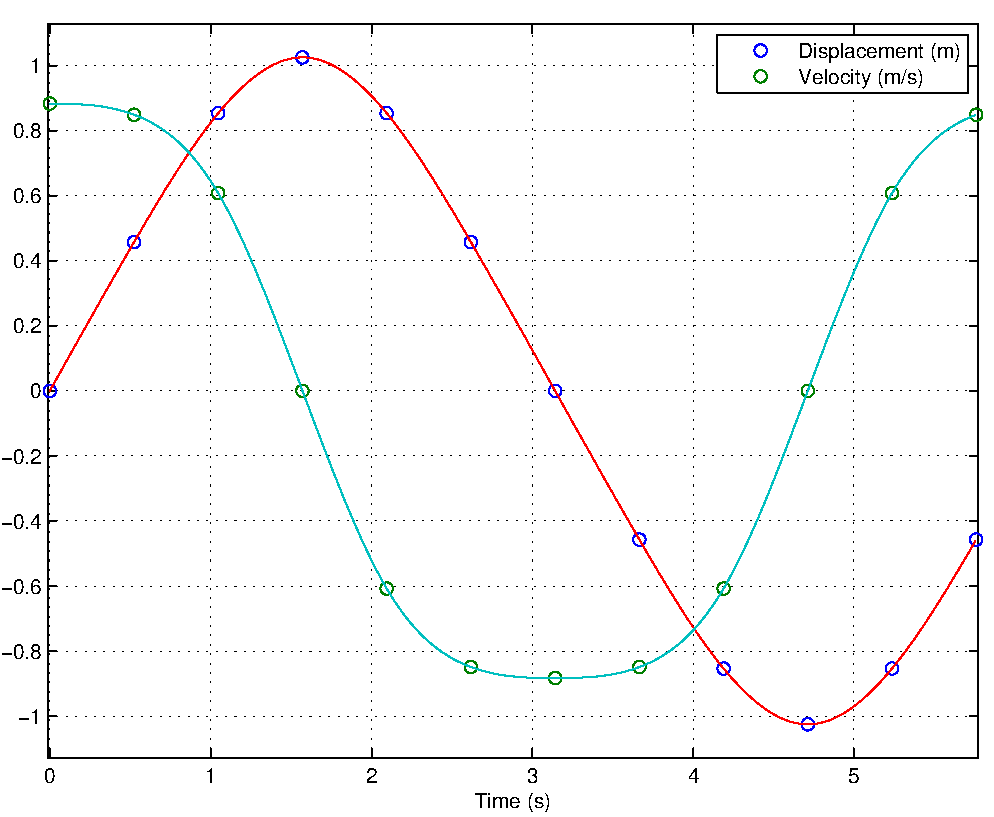
\includegraphics[width=.45\textwidth]{WSUThesisTemplate/pix/example.pdf}}
%   \subfigure[Second sub-figure]{
%\label{fig:example_b}
%   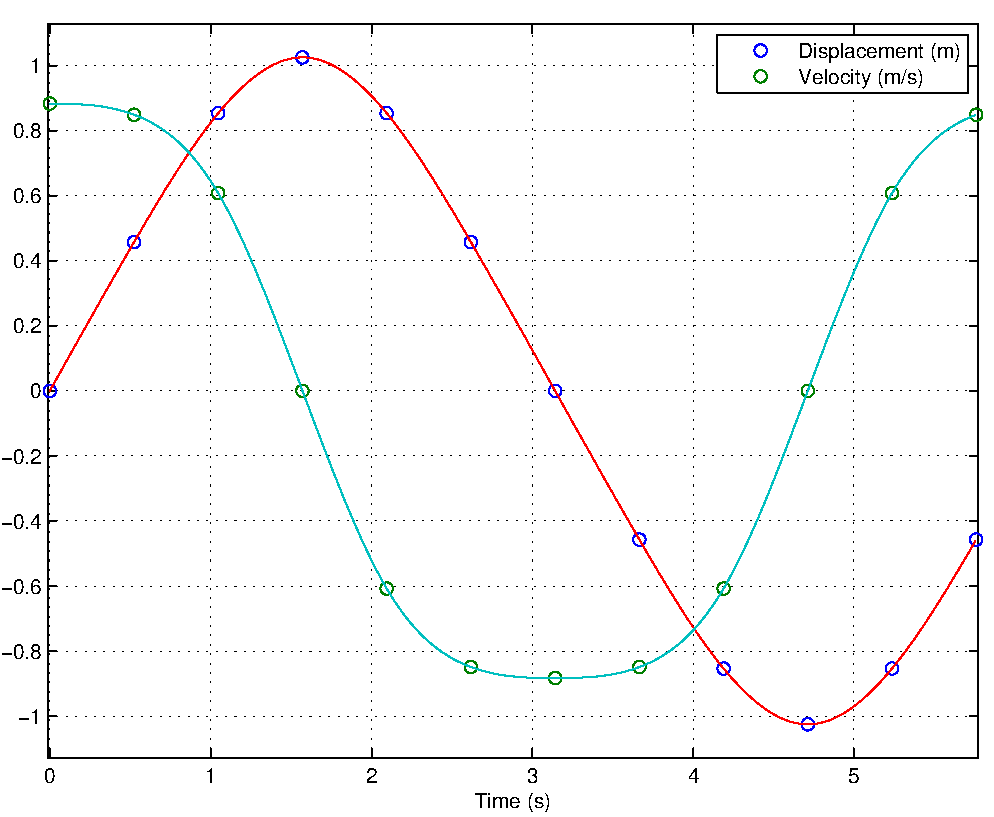
\includegraphics[width=.45\textwidth]{WSUThesisTemplate/pix/example.pdf}}
%   \caption{Side-by-side sub-figures.}
%\label{fig:1x2_subfigs}
%\end{figure}
%%-----------------------------------------------------------------
%
%
%If you want 4 total figures, just add a line break, \verb'\\', after the second sub-figure as shown in Figure~\ref{fig:2x2_subfigs}.  You can add spacing between them with the \verb'\quad' or \verb'\qquad' commands.  There is more space between Figures~\ref{fig:example_2x2a} and~\ref{fig:example_2x2b} to show the use of this spacing.  Make sure all of your spacing is equal.  And don't make your figures too small.  As my advisor told me, ``old people read these''\cite{Mark}.
%
%%-----------------------------------------------------------------
%\begin{figure}[!t]
%   \centering
%   \subfigure[First sub-figure]{
%\label{fig:example_2x2a}
%   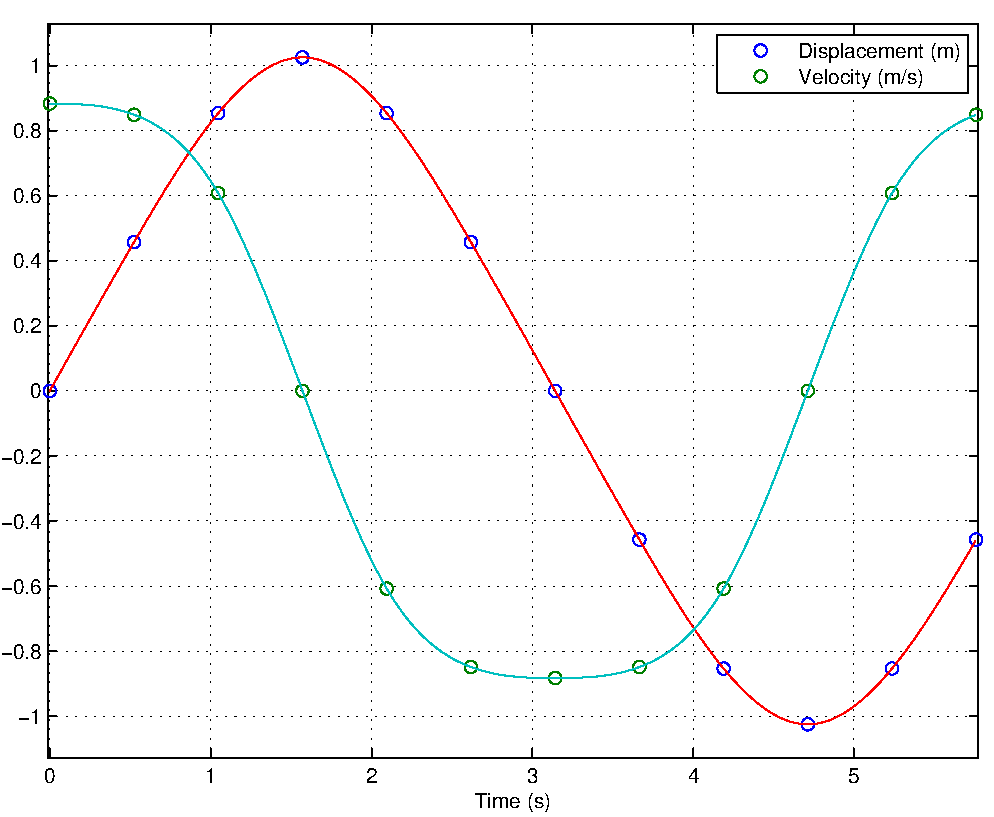
\includegraphics[width=.25\textwidth]{WSUThesisTemplate/pix/example.pdf}} \quad
%   \subfigure[Second sub-figure]{
%\label{fig:example_2x2b}
%   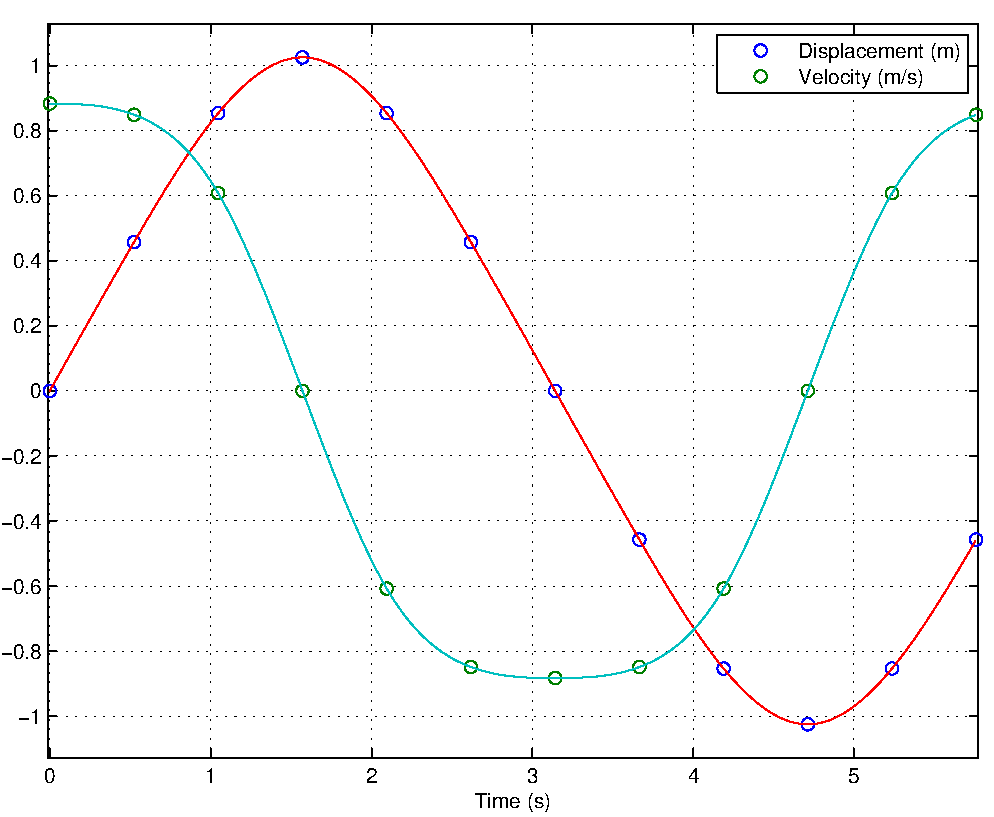
\includegraphics[width=.25\textwidth]{WSUThesisTemplate/pix/example.pdf}}\\
%      \subfigure[Third sub-figure]{
%\label{fig:example_2x2c}
%   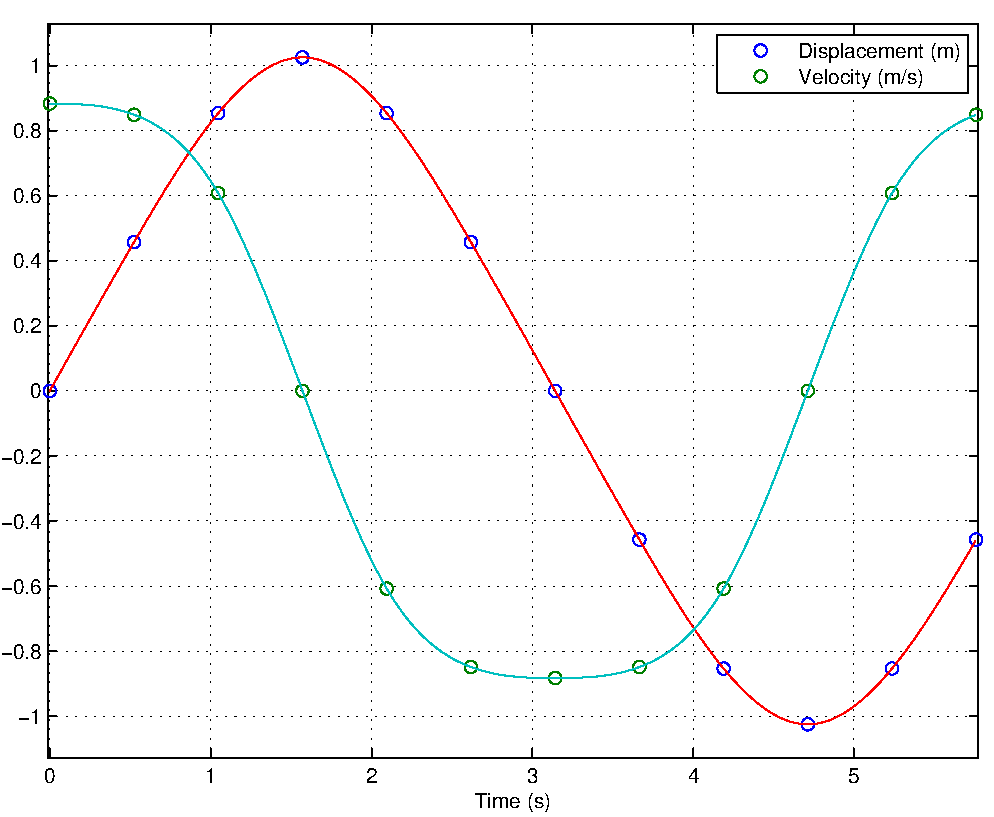
\includegraphics[width=.25\textwidth]{WSUThesisTemplate/pix/example.pdf}}
%   \subfigure[Fourth sub-figure]{
%\label{fig:example_2x2d}
%   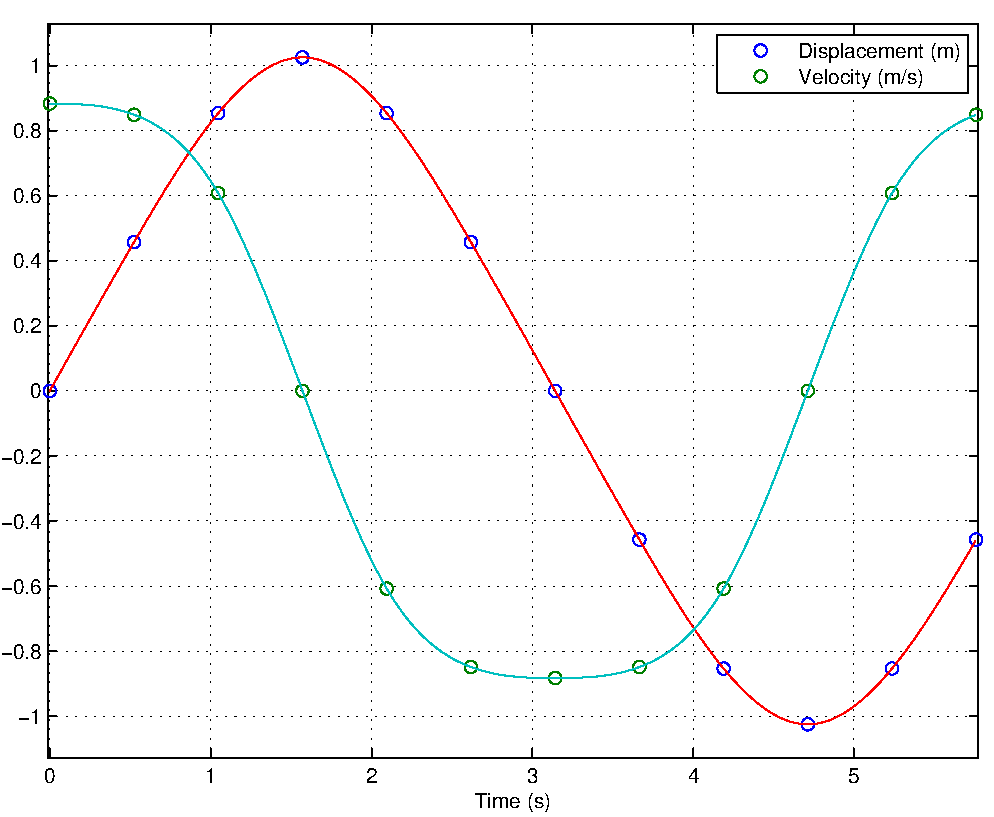
\includegraphics[width=.25\textwidth]{WSUThesisTemplate/pix/example.pdf}}
%\caption{2$\times$2 sub-figures.}
%\label{fig:2x2_subfigs}
%\end{figure}
%%-----------------------------------------------------------------
%
%%=============================
%\section{Including Chapters or Files}
%%=============================
%You can include chapters using the \verb'\include' command. See the \LaTeX\ file.  Each file can be included separately as to keep editing localized to each chapter.
%% ------------------------------------------------------------------------
%%\include{chapter2}
%% ------------------------------------------------------------------------
%%\include{chapter3}
%% ------------------------------------------------------------------------
%
%You can also use the \verb'\input' command to include items without forcing a page break.  This becomes handy when generating a table, you can leave the reference in the main document and the table can be updated separately.
%\begin{table}[ht] % h - here, t - top, b - bottom, p - page (use a ! to force the table for figure where you want)
  \centering
  \scriptsize % set font size to scriptsize so that table fits within page margins
  \caption{Complete test matrix of waveforms for experimental bench test}
    \begin{tabular}{cccccc}
    \toprule % top line of table
    \textbf{Bandwidth} & \textbf{FFT lines} & \textbf{Samples/Cycle Chirp} & \textbf{Frequency Resolution} & \textbf{Sweep Rate} & \textbf{Sweep Time} \\
	(Hz) 	& 		&	 		& (mHz) & (mHz/sec)	& (sec) \\ \midrule
\multirow{4}[8]{.5in}{\centering8}
		& 100		& 3-10, 20 		& 80    	& 0.64		& 12.5 \\ \cmidrule (l){2-6} % midrule between columns 2-6
		& 200		& 3-10 	     		& 40
                                                                                                           & 0.32 		& 25 \\ \cmidrule (l){2-6}
		& 400   	& 3-10  		& 20   	& 0.16  	& 50 \\ \midrule
%
\multirow{5}[8]{.5in}{\centering16}
		& 100   	& 3-10, 20, 50      	& 160   & 2.56  	& 6.25 \\ \cmidrule (l){2-6}
		& 200   	& 3-10, 20		& 80    	& 1.28  	& 12.5 \\ \cmidrule (l){2-6}
		& 400   	& 3-10, 20     		& 40    	& 0.64  	& 25 \\ \cmidrule (l){2-6}
		& 800		& 3-10      		 & 20    & 0.32  	& 50 \\ \midrule
%
\multirow{6}[12]{.5in}{\centering32}
		& 100   	& 3-10, 20     		 & 320	& 10.24 	& 3.125 \\ \cmidrule (l){2-6}
		& 200   	& 3-10, 20      		& 160	& 5.12  	& 6.25 \\ \cmidrule (l){2-6}
		& 400   	& 3-10, 20      		& 80	& 2.56  	& 12.5 \\ \cmidrule (l){2-6}
		& 800   	& 3-10, 20      		& 40	& 1.28 	 	& 25 \\ \cmidrule (l){2-6}
		& 1600  	& 3-10       		& 20	& 0.64  	& 50 \\ \bottomrule % bottom line of table
    \end{tabular}
\label{tab:bench_test_matrix}
  \normalsize % reset font size to normal
\end{table}

%
%Using the \verb'booktabs' package makes very professional looking tables by varying the thickness of the lines which can be customized.
%
%%=============================
%\clearpage \section{Inserting Code}
%%=============================
%If you want to insert code into your document by reference, instead of copy/paste, you even use the \href{https://en.wikibooks.org/wiki/LaTeX/Source_Code_Listings}{listings} package.  
%
%\href{http://www.mathworks.com}{Matlab} users may find the simpler interface of the \verb'mcode' package easier.  To do that simply comment the \verb'\usepackage{listings}' line near the top of this (the \verb'.tex') document and uncomment the preceding line. You can choose to between several options to frame, have numbered lines, automatic line breaks and more.  Below is an example of listing a MATLAB\textsuperscript{\textregistered} m-file.
%
%\lstinputlisting[language=matlab, basicstyle=\linespread{1}\normalsize]{WSUThesisTemplate/importfile.m}
%
%%=============================
%\chapter[Programs]{Typesetting Programs using \LaTeX\ }
%%=============================
%\section{Windows}
%%=============================
%Below are some programs for Windows:
%\begin{itemize}
%\item \href{http://miktex.org/}{MiK\TeX}
%\subitem- Up-to-date implementation of \TeX\
%\subitem- Side-by-side comparison of source and PDF
%\subitem- Has portable version that can be run from portable storage device
%\item \href{http://www.lyx.org/}{LyX}
%\subitem- Graphical interface used with \TeX\ and \LaTeX\
%\item \href{http://www.tug.org/texlive/}{\TeX Live} (also Unix)
%\item \href{http://www.tug.org/protext/}{pro\TeX t}
%\end{itemize}
%
%%=============================
%\section{Mac OS}
%%=============================
%Below are some programs for Mac OS:\@
%\begin{itemize}
%\item \href{http://www.lyx.org/}{LyX}
%\item\href{http://www.tug.org/mactex/}{Mac\TeX}
%\subitem- \TeX\ Live with the addition of Mac specific programs
%\item gw\TeX\   (Mac OS X)
%\item Latexian (Mac OS X)
%\end{itemize}
%
%\section{References}
%\label{sec:refs}
%\begin{itemize}
%\item \href{http://www.ctan.org}{CTAN} home page
%\item \href{http://en.wikibooks.org/wiki/LaTeX/}{Wikibooks} \LaTeX\ home page
%\end{itemize}


%
%
%-----------------------------------------------------------------------
% Bibliography
%-----------------------------------------------------------------------
\clearpage \phantomsection\ %used to correctly anchor hyperlinks, just
                           %trust us and leave it alone.
\renewcommand\baselinestretch{1.0}
\addcontentsline{toc}{chapter}{Bibliography}
\bibliographystyle{plain}
\bibliography{references}
%
%-----------------------------------------------------------------------
% Appendices
%-----------------------------------------------------------------------
%%%%%%%%%%%%%%%%%%%
\begin{appendices}
\phantomsection\ %use \phantomsection command to correctly anchor hyperlinks
\chapter[An Example Appendix]{Appendix A\\An Example}
\label{chap:AppA}
Here is an appendix\ldots not too difficult.
\phantomsection\
\chapter[Another Example Appendix]{Appendix B\\Another Example}
\label{chap:AppB}
Again\ldots not too difficult.
\end{appendices}
%%%%%%%%%%%%%%%%%%%
%
%
%
% End of document
\end{document}

%%% Local Variables:
%%% mode: latex
%%% TeX-master: "WSUThesisTemplate"
%%% End:
